\begin{frame}{Implementation}
%     \bbsp \ip Need to monitor, report and verify emissions of industrial units.
%         \bbsp \ip Challenging to avoid fraud in countries lacking institutional capacity, but same for any climate policy.
%         \ip The GCP would provide resources and assistance from experienced countries. \ee
%     \ip Distributing a global basic income is challenging: need to reach everyone and avoid fraud.
%         \bbsp \ip Most countries maintain electoral lists and already have social programs for isolated people.
%         \ip Smartphones can provide biometric identification and means of transaction.
%         \ip Satellite internet access might soon become cheap and ubiquitous (Hanson 2016).
%         \ee
%     \ee 
% \end{frame}

% \begin{frame}{Details}
%     \bbsp \ip \textbf{Ideal timeline}: negotiation, consultations up to 2030, phase-in between 2030 and 2035.
%     \ip \textbf{Scope}: ideally, all CO$_\text{2}$. Initially, CO$_\text{2}$ from fossil fuels and cement production in large industrial units, including shipping and aviation.
%     \ip \textbf{Framework}: defines the scope, use of revenues, rules of governance, and \blue{carbon budget} (e.g. 500 GtCO$_\text{2}$ 
%     $\approx$ $<+1.5$\textdegree{}C with 50\% chance). %500 GtCO$_\text{2}$ from 2030  $\approx$ $<+2$\textdegree{}C with 67\% chance).
%     \ip \textbf{Governance}: the governing body would choose the yearly emissions quota, the market design, and possible sanctions against non-participating or non-complying entities. % Voting rights proportional to emissions
%     \ip \textbf{Market design}: Carbon offsets should not be allowed. Borrowing and banking emissions permits should be limited.
%     \ee
% \end{frame}

% % \begin{frame}{Let's continue the discussion}
% %     \begin{figure}
% %         \centering \caption{You liked the GCP? \href{https://github.com/bixiou/global_tax_attitudes/raw/main/paper/policy_brief_GCS.pdf}{Read}, share, endorse on \rose{\href{https://global-redistribution-advocates.org/the-global-climate-plan/}{global-redistribution-advocates.org}}!}
% %         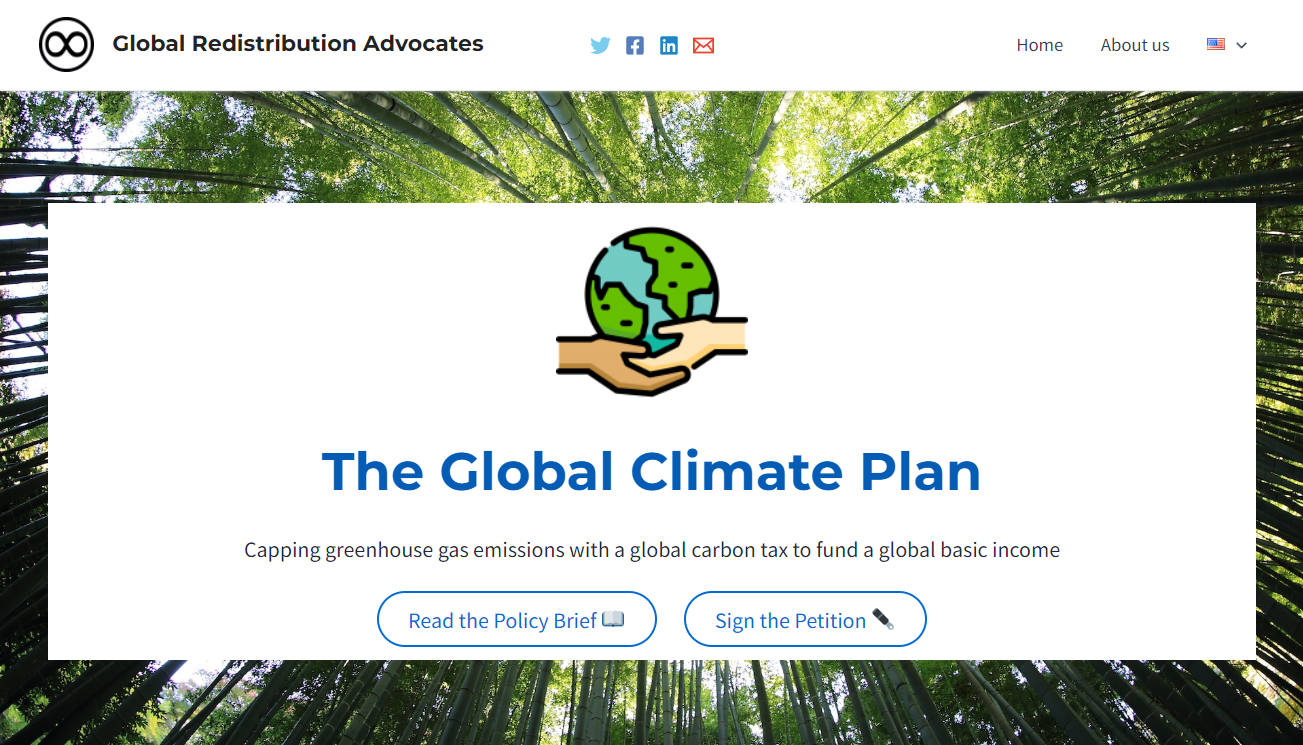
\includegraphics[height=.55\textheight]{../figures/policies/petition.PNG} 
% %     \end{figure}    
% %     \bbsp \ip \quad \quad \quad \quad \quad \quad Want to help? \pause We need specialists for the GCP's scientific committee.
% %     \ip \pause \quad \quad \quad \quad \quad \quad Have comments or criticisms? \pause Happy to take any question or remark!
% %     \ip \hspace{6.5cm} \href{https://youtu.be/Bypt4H8K5dI?t=106s}{\beamergotobutton{Video}}
% %     \ee
% % \end{frame}

% \appendix
% \section{Appendix}

% \subsection{Additional results}

% % TODO appendix
% % \begin{frame}{Support for increased foreign aid\label{}}\vspace{-.2cm} 
% %     \begin{figure} 
% %         \centering 
% %         \caption{Actual, perceived and preferred amount of foreign aid, with random info (or not) on actual amount. (\textit{Mean})}\vspace{-.2cm}
% %         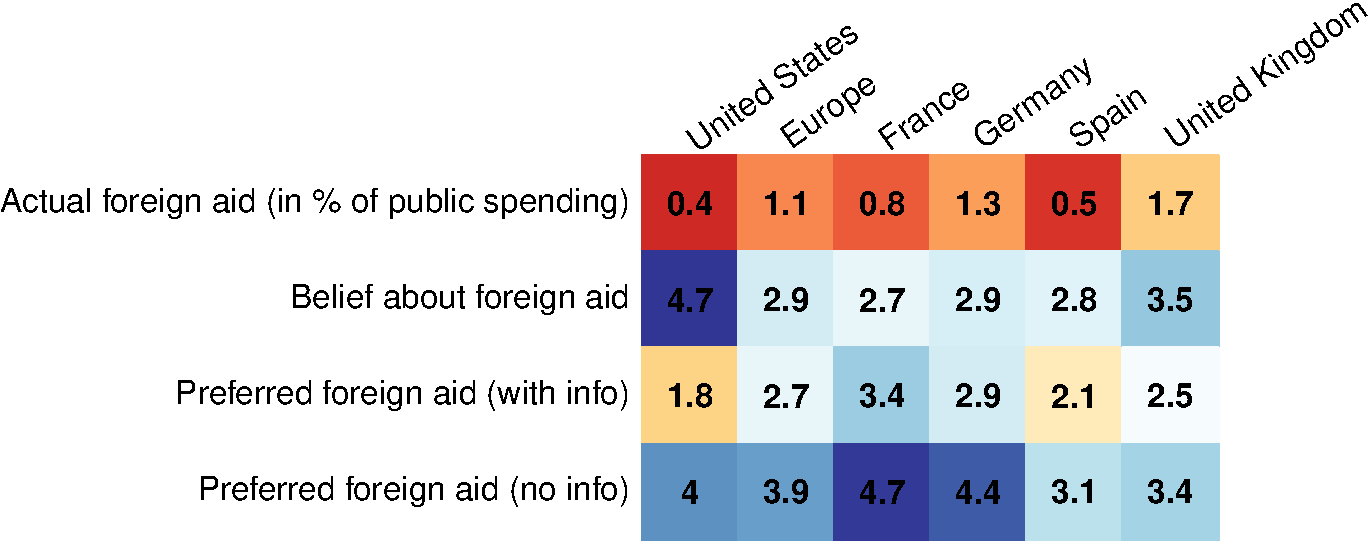
\includegraphics[height=.4\textheight]{../figures/country_comparison/foreign_aid_amount_mean.pdf} % TODO: see median
% %     \end{figure}\vspace{-.2cm}\pause
% %     \begin{figure} 
% %         \centering 
% %         % \caption{Support for increased foreign aid (vs. reduced or stable): from previous question, and directly asked (with info).}\vspace{-.2cm}
% %         % 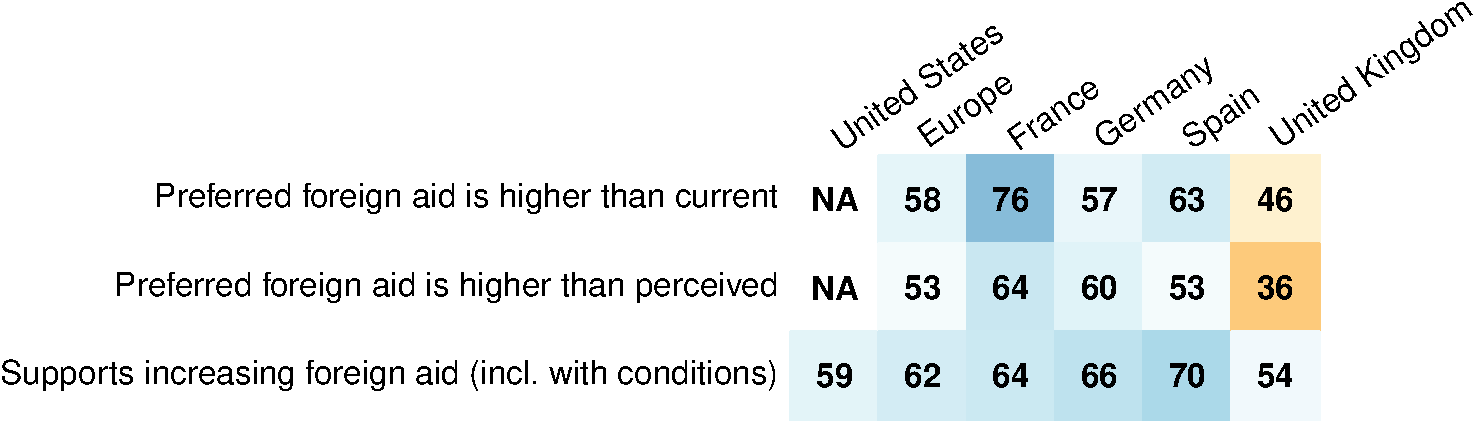
\includegraphics[height=.32\textheight]{../figures/country_comparison/foreign_aid_more_positive.pdf} 
% %         \caption{Support for increased foreign aid: from previous question, and directly asked (with info).}\vspace{-.2cm}
% %         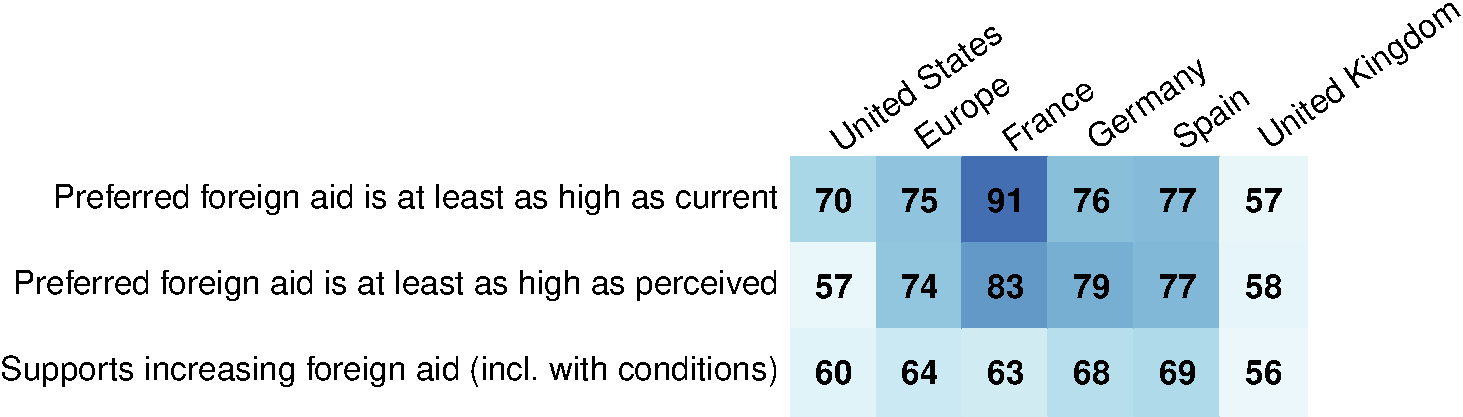
\includegraphics[height=.32\textheight]{../figures/country_comparison/foreign_aid_no_less_positive.pdf} 
% %     \end{figure} \vspace{-.1cm}
% % 	\quad \quad \quad \quad \quad \quad \blue{Actual foreign aid is overestimated.} \quad \quad \quad \rose{Majorities support more foreign aid.}
% % \end{frame}

% \begin{frame}{Conditions for increased foreign aid \label{foreign_aid_conditions} \hyperlink{other_policies}{\beamergotobutton{Go back}}}
%     \begin{figure} \vspace{-.2cm}
%         \centering 
%         \caption{[Info on actual amount]. Do you support [the U.S.] transferring more money to low-income countries?}\vspace{-.2cm}
%         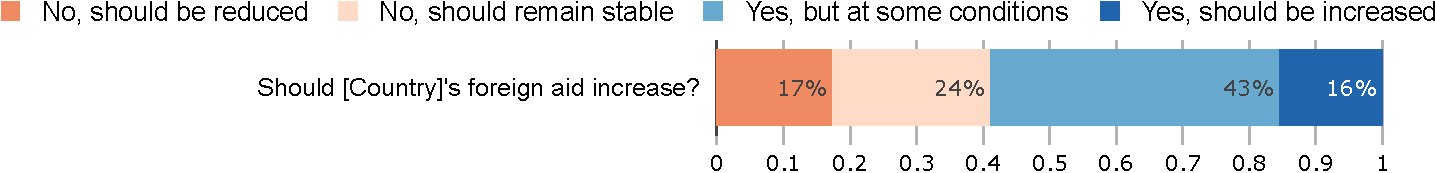
\includegraphics[width=.7\textwidth]{../figures/all/foreign_aid_raise_support.pdf} 
%     \end{figure}\vspace{-.2cm} \pause
%     \begin{figure} 
%         \centering 
%         \caption{[If \textit{at some conditions}] What conditions should be required for [the U.S.] to increase its foreign aid?}\vspace{-.2cm}
%         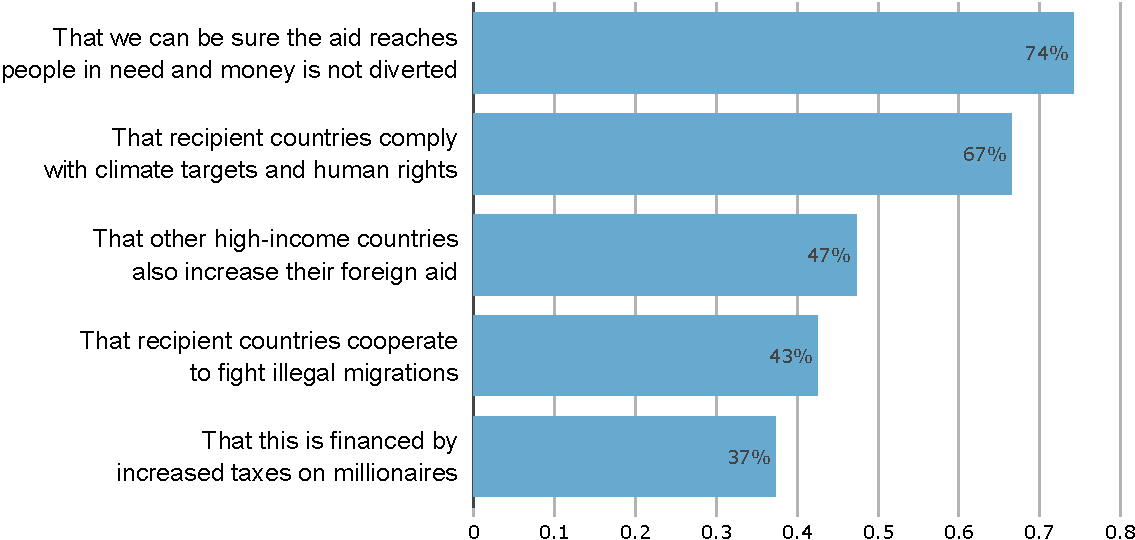
\includegraphics[height=.48\textheight]{../figures/all/foreign_aid_condition.pdf} 
%     \end{figure} \pause \vspace{-.3cm}
% 	\bbvs \ip \blue{People want to help people (not oligarchs) and to foster climate action and human rights.}% sustainability.
% 	\ip National preference is the main reason behind not wanting increased foreign aid.
% 	\ee 
% \end{frame}

% \begin{frame}{Preferences over public spending%How to fund increased foreign aid
% 	\hyperlink{other_policies}{\beamergotobutton{Go back}}}
% 	\begin{columns}
%         \begin{column}{0.5\textwidth}
%             \begin{figure}
% 				\vspace{-.2cm}
%                 \centering 
%                 \caption{Your previous answer shows that you would like to increase [UK] foreign aid.\\How would you like to finance such increase in foreign aid? (Multiple answers possible)}
%                 \vspace{-.2cm}
%                 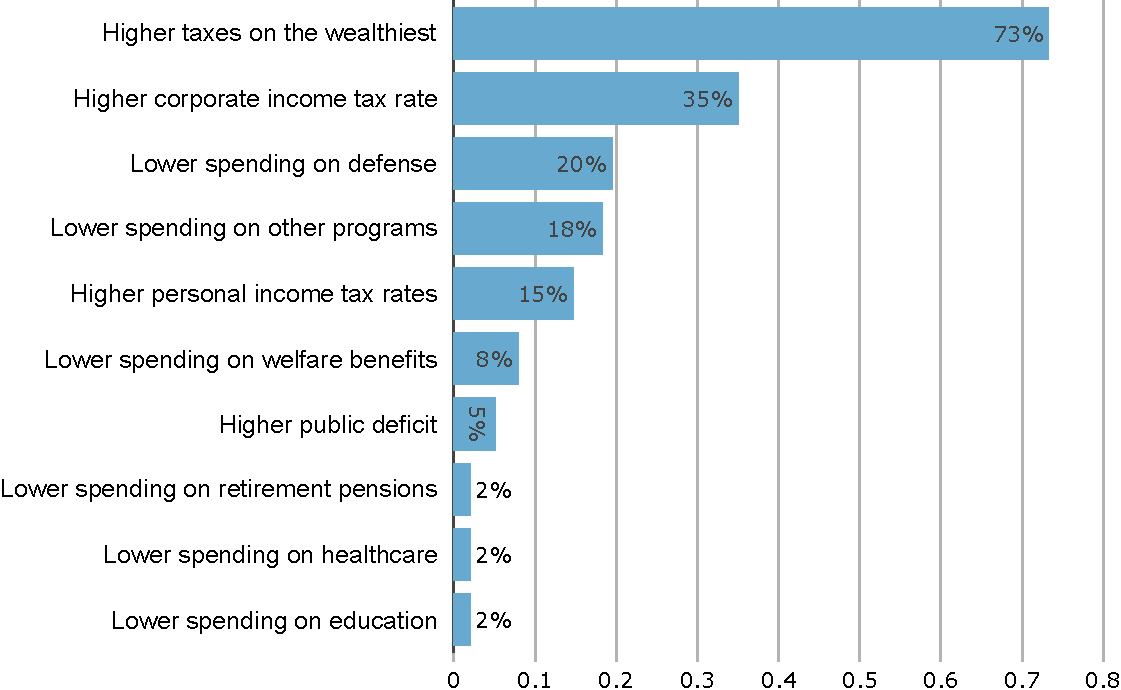
\includegraphics[width=\columnwidth]{../figures/all/foreign_aid_raise.pdf} 
%             \end{figure}
%         \end{column}
%         \begin{column}{0.5\textwidth}			
%             \begin{figure}\vspace{-.2cm}
%                 \centering 
%                 \caption{Your previous answer shows that you would like to reduce [UK] foreign aid.\\How would you like to use the freed budget? (Multiple answers possible)}
%                 \vspace{-.2cm}
%                 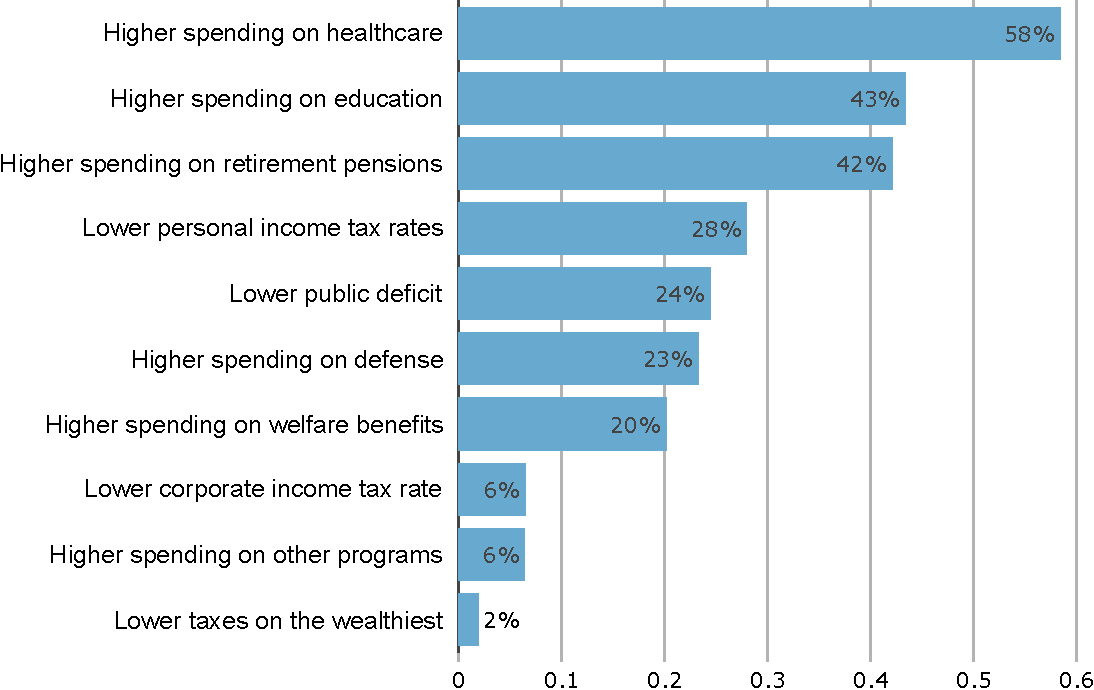
\includegraphics[width=\columnwidth]{../figures/all/foreign_aid_reduce.pdf} 
%             \end{figure}
%         \end{column}
%     \end{columns}
% 	\bbvs \ip \rose{People want better public services and higher taxes on the wealthiest.}
% 	\ee 
% \end{frame} 

% \begin{frame}{Support for increased foreign aid \hyperlink{other_policies}{\beamergotobutton{Go back}}\label{foreign_aid_perceptions}}\vspace{-.2cm} 
%     \begin{figure} 
%         \centering 
%         \caption{Actual, perceived and preferred amount of foreign aid, with random info (or not) on actual amount. (\textit{Mean})}\vspace{-.2cm}
%         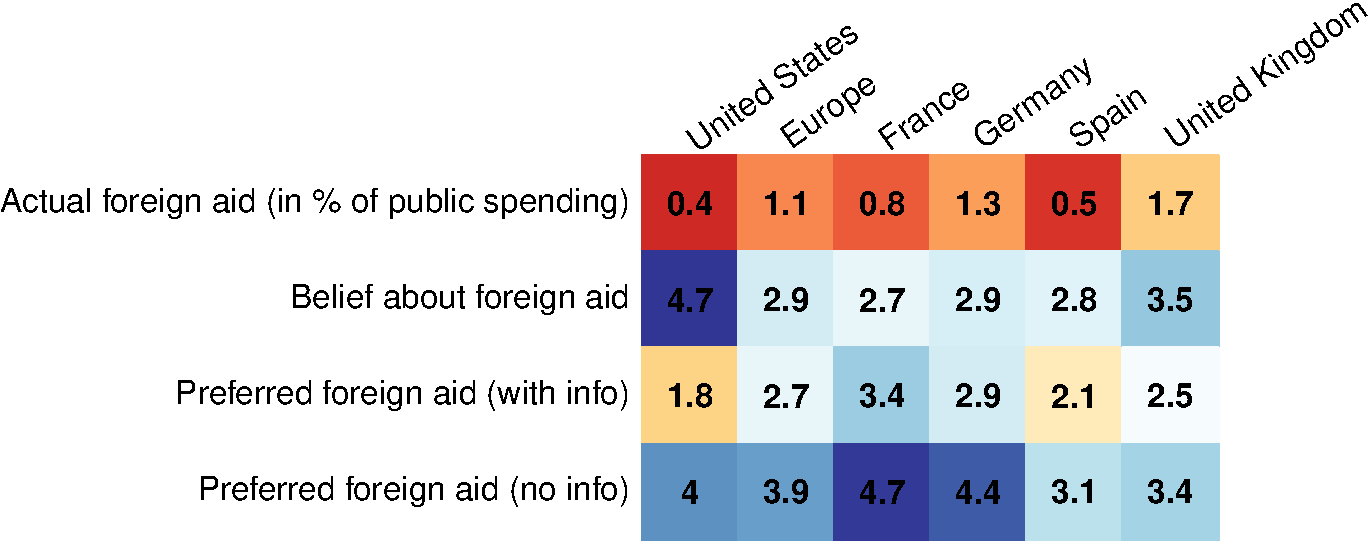
\includegraphics[height=.4\textheight]{../figures/country_comparison/foreign_aid_amount_mean.pdf} % TODO: see median
%     \end{figure}\vspace{-.2cm}\pause
%     \begin{figure} 
%         \centering 
%         % \caption{Support for increased foreign aid (vs. reduced or stable): from previous question, and directly asked (with info).}\vspace{-.2cm}
%         % 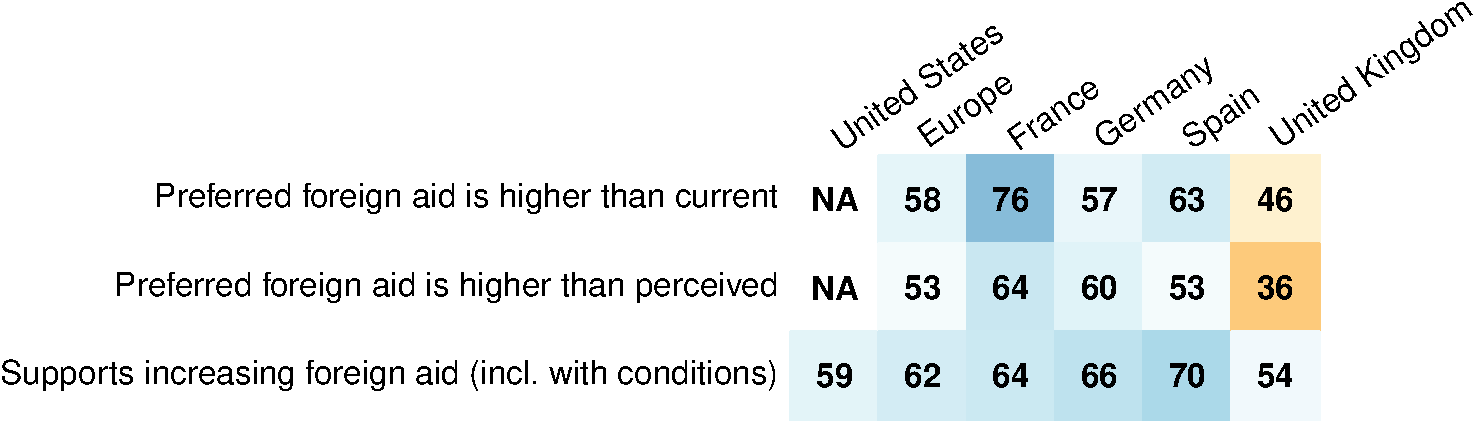
\includegraphics[height=.32\textheight]{../figures/country_comparison/foreign_aid_more_positive.pdf} 
%         \caption{Support for increased foreign aid: from previous question, and directly asked (with info).}\vspace{-.2cm}
%         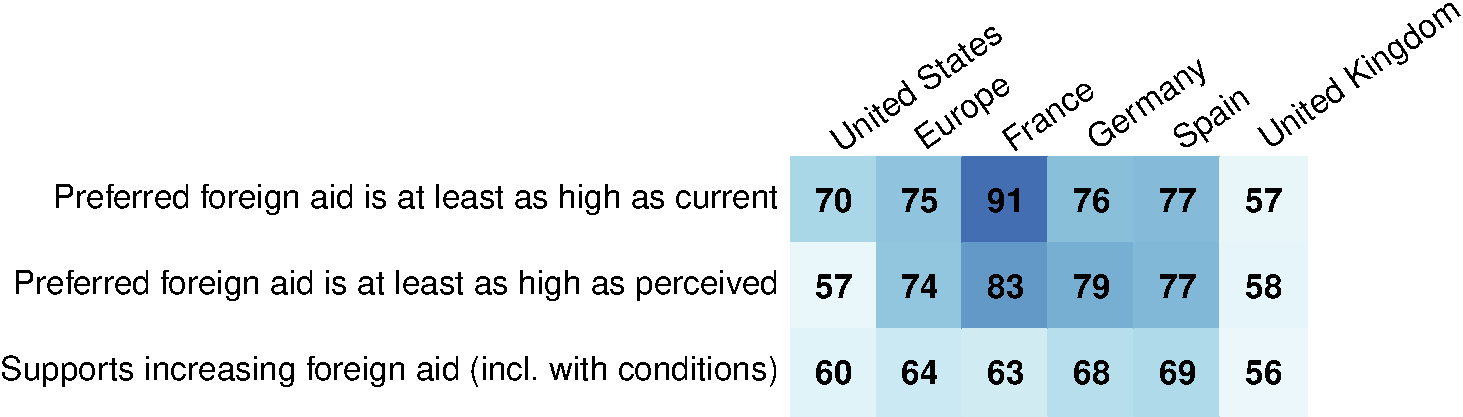
\includegraphics[height=.32\textheight]{../figures/country_comparison/foreign_aid_no_less_positive.pdf} 
%     \end{figure} \vspace{-.1cm}
% 	\quad \quad \quad \quad \quad \quad \blue{Actual foreign aid is overestimated.} \quad \quad \quad \rose{Majorities support more foreign aid.}
% \end{frame}

% \begin{frame}{Perceptions of the Global Climate Scheme \hyperlink{gcs_support}{\beamergotobutton{Go back}}\label{gcs_perceptions}}
% 	\vspace{-.3cm}
%     \begin{figure}
%         \centering 
%         \caption{When determining your support or opposition to the Global climate scheme, which points are important to you?}
%         \vspace{-.2cm}
%         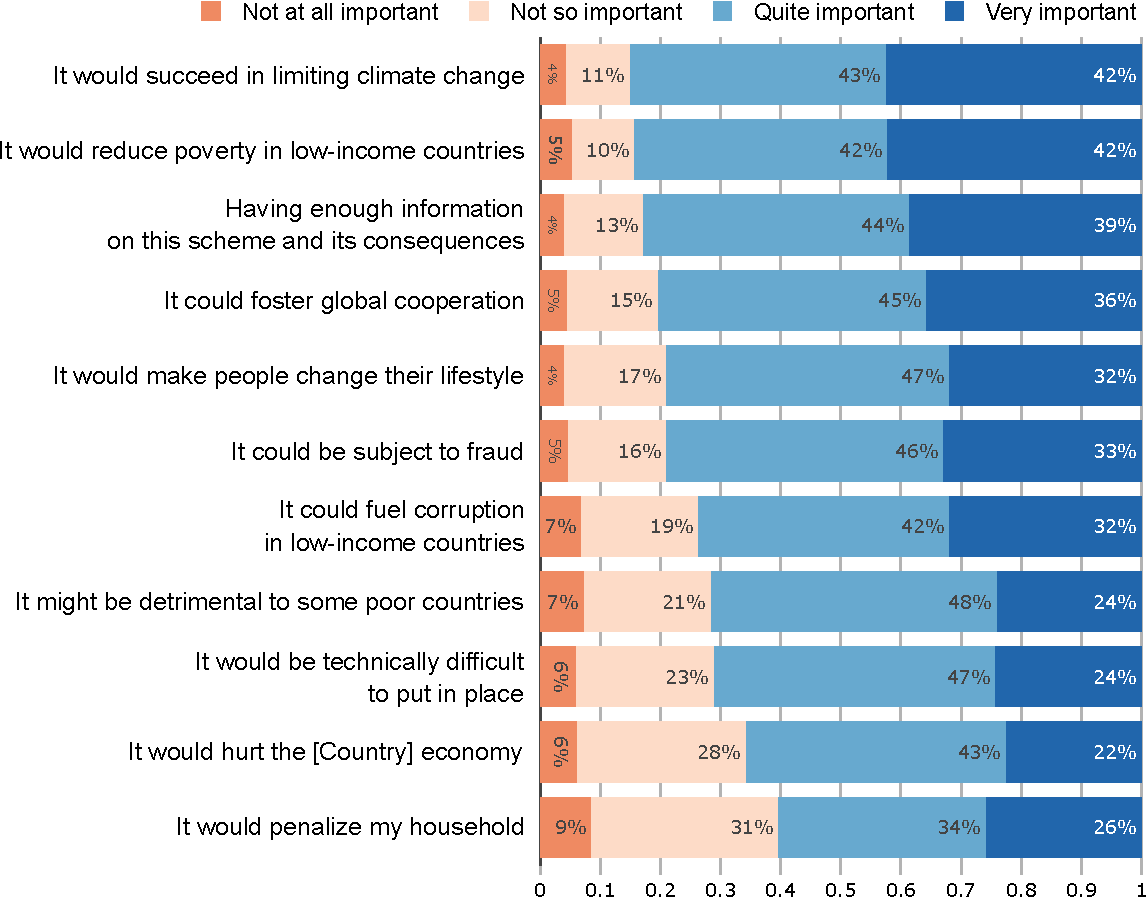
\includegraphics[height=.9\textheight]{../figures/all/gcs_important.pdf} 
%     \end{figure}
% \end{frame}

% \begin{frame}{Conjoint analyses: interaction with other policies \hyperlink{gcs_support}{\beamergotobutton{Go back}}\label{conjoint_ab}} 
%     \bbvs \ip National climate policy (C) is as supported as the GCS, but no substitute for it.
% 	\ip Support for the GCS does not increase when complemented by National Redistribution.
% 	\ip $\Rightarrow$ Confirms that the \rose{monetary loss is not a primary concern} for one's attitude toward the GCS.
%     \ee
%     \begin{figure} \vspace*{-.5cm}
%         \centering 
%         \caption{Among the two following bundles of policies, which one would you prefer?}
%         \vspace{-.2cm} 
%         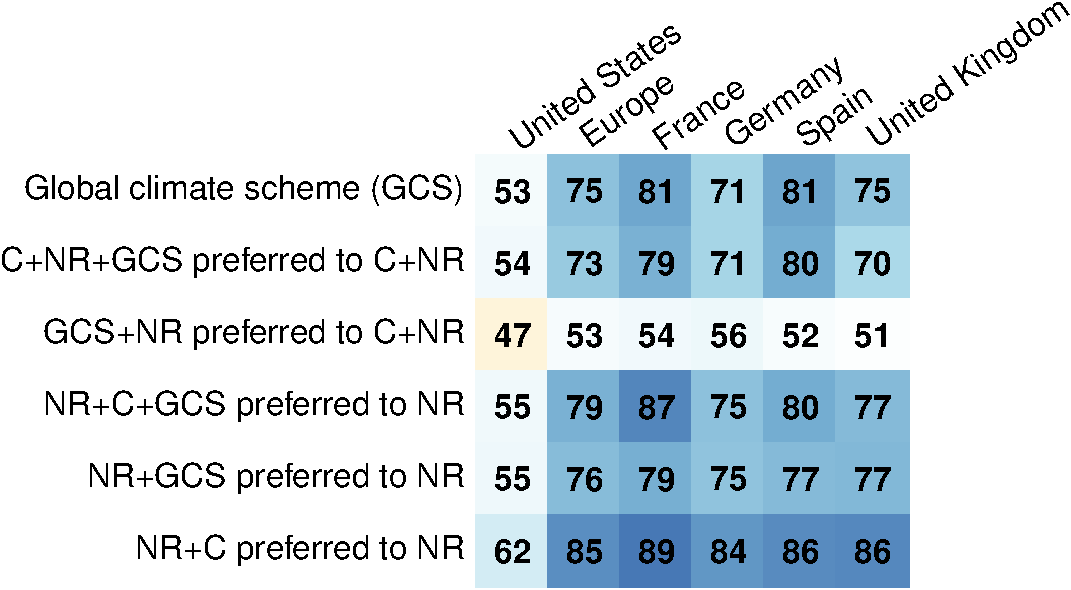
\includegraphics[height=.65\textheight]{../figures/country_comparison/conjoint_ab_positive.pdf} 
%     \end{figure}
% \end{frame}

% \begin{frame}{Conjoint analyses: influence on preferred platform (Eu) \hyperlink{conjoint_r_uk}{\beamergotobutton{Go back}}\label{conjoint_r_eu}} 
%     \begin{figure}\vspace{-.2cm}
%         \centering 
%         \caption{%Imagine that a [Left or Center-left coalition wins the next elections]. Here are two possible platforms on which [the coalition] may campaign (the policies in each platform are randomly drawn from a pool of credible [Left/Center-left] policies).\\
% 		(...) Even if you do not support the Left, which of these platforms do you prefer? 
% 		%\\ ~[FR: Left or center-left; DE: rot-rot-grüne; ES: PSOE; UK: Labour]
% 		}
%         \vspace{-.2cm} 
%         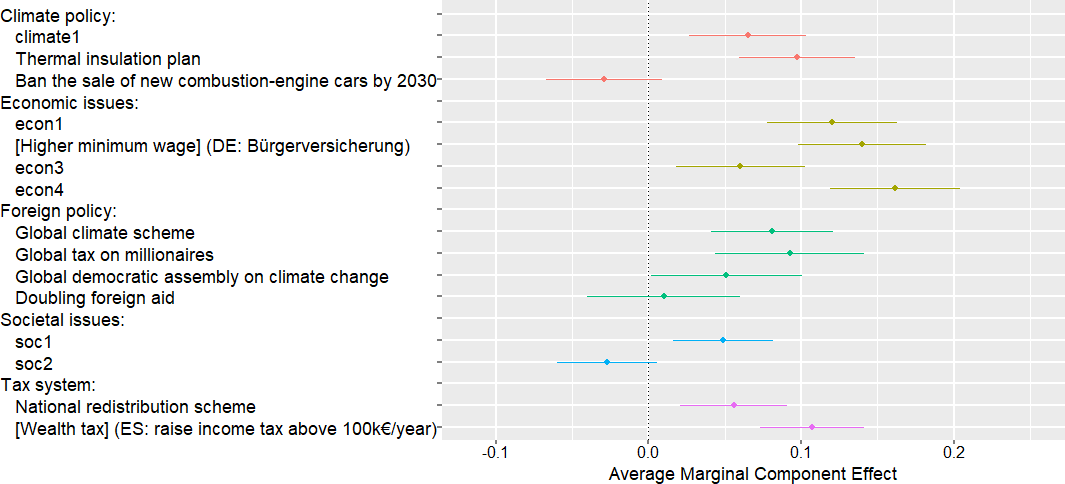
\includegraphics[height=.7\textheight]{../figures/EU/ca_r.png} 
%     \end{figure}
%     \bbvs \ip \rose{Europeans prefer platforms that include the GCS} and without the ban on thermal cars (a planned policy).
% 	\ip The effect of GCS is among the highest (wealth tax, better public services, higher minimum wage).
%     \ee
% \end{frame}

% \begin{frame}{Conjoint analyses: influence on preferred platform (France)\label{conjoint_r_fr} \hyperlink{conjoint_r_uk}{\beamergotobutton{Go back}}} 
% 	\vspace{-.2cm}
%     \bbvs \ip France shows that there can be a \rose{mismatch between preferred} policies (insulation plan, public services, global tax, GCS) \rose{and enacted policies} (higher retirement age and ban on thermal cars: the least preferred).
%     \ee
%     \begin{figure}\vspace{-.4cm}
%         \centering 
%         \caption{Imaginez que la gauche ou le centre gauche gagne les prochaines élections en 2027. Voici deux programmes possibles sur lesquels elle pourrait faire campagne (...)%(les mesures de ces programmes sont tirés aléatoirement depuis un ensemble de mesures de gauche ou centre gauche).
% 		%\\ Même si vous n'êtes pas de gauche ou centre gauche
% 		, lequel de ces programmes préférez-vous ?}
%         \vspace{-.2cm} 
%         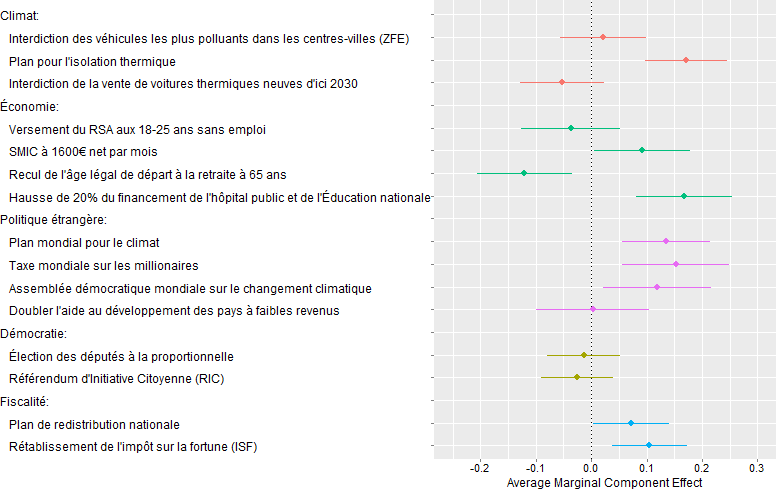
\includegraphics[height=.7\textheight]{../figures/FR/ca_r.png} 
%     \end{figure}
% \end{frame}

% \begin{frame}{Conjoint analyses: influence on preferred platform (U.S.) \hyperlink{conjoint_r_uk}{\beamergotobutton{Go back}}\label{conjoint_r_us}} 
%     \bbvs \ip \rose{Endorsing the GCS is not determinant to gain the Democratic primary.}
%     \ee
%     \begin{figure}\vspace{-.4cm}
%         \centering 
%         \caption{[Only on non-Republican] Imagine that at the 2024 Democratic party presidential primaries, the two main candidates campaign with the following key policies in their platforms.\\
% 		Which of these candidates do you prefer?}
%         \vspace{-.2cm} 
%         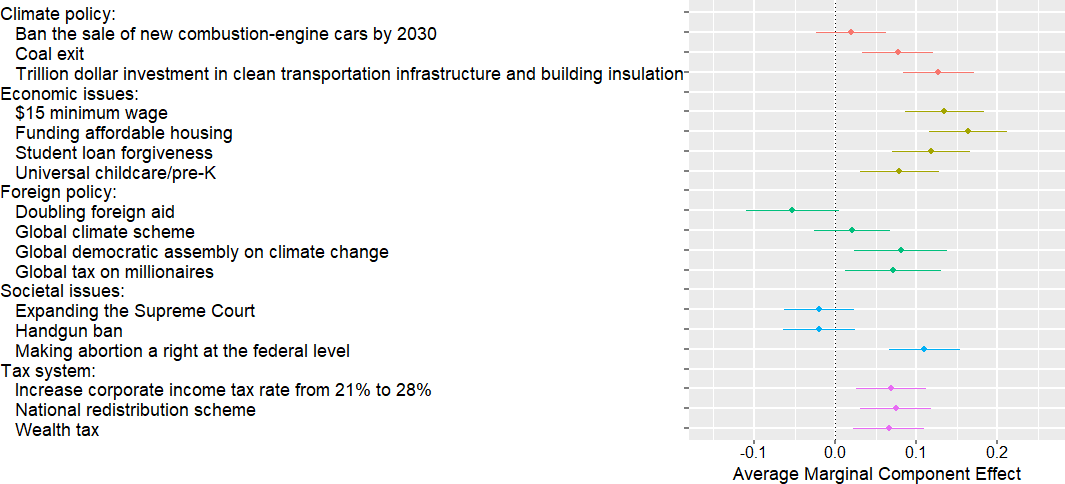
\includegraphics[height=.7\textheight]{../figures/US1/ca_r.png} 
%     \end{figure}
% \end{frame}

% \begin{frame}{Conjoint analyses: influence on preferred platform (Germany) \hyperlink{conjoint_r_uk}{\beamergotobutton{Go back}}\label{conjoint_r_de}} 
%     \bbvs \ip \rose{Endorsing the GCS is not determinant to gain the Democratic primary.}
%     \ee
%     \begin{figure}\vspace{-.4cm}
%         \centering 
%         \caption{Imagine that a Rot-Rot-Grüne coalition wins the next elections. Here are two possible platforms on which the coalition may campaign (the policies in each platform are randomly drawn from a pool of credible left-wing policies).\\
% 		(...) Even if you do not support the Left, which of these platforms do you prefer? }
%         \vspace{-.2cm} 
%         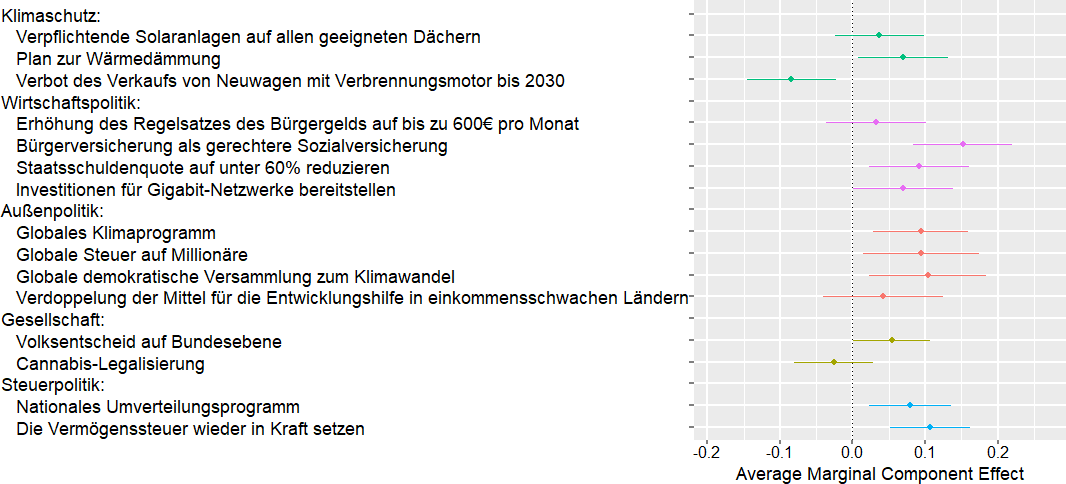
\includegraphics[height=.7\textheight]{../figures/DE/ca_r.png} 
%     \end{figure}
% \end{frame}

% \begin{frame}{Conjoint analyses: influence on preferred platform (Spain) \hyperlink{conjoint_r_uk}{\beamergotobutton{Go back}}\label{conjoint_r_es}} 
%     \bbvs \ip \rose{Endorsing the GCS is not determinant to gain the Democratic primary.}
%     \ee
%     \begin{figure}\vspace{-.4cm}
%         \centering 
%         \caption{Imagine that the PSOE wins the next elections. Here are two possible platforms on which it may campaign (the policies in each platform are randomly drawn from a pool of credible PSOE policies).\\
% 		(...) Even if you do not support the PSOE, which of these platforms do you prefer? }
%         \vspace{-.2cm} 
%         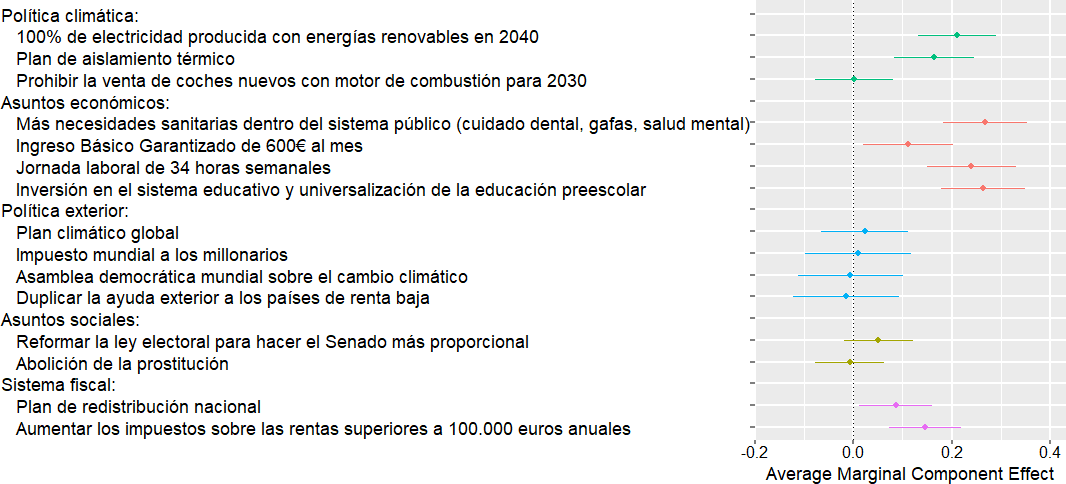
\includegraphics[height=.7\textheight]{../figures/ES/ca_r.png} 
%     \end{figure}
% \end{frame}

% \begin{frame}{Prioritization \hyperlink{donation}{\beamergotobutton{Go back}}\label{prioritization}}
%     \begin{columns}
%         \begin{column}{0.35\textwidth}\vspace{-1cm}
%             \bbvs \ip %``In this question, 
% 			``you have 100 points that you can allocate to different policies. The more you give points to a policy, the more you support it.\\ % TODO: highlight synchronously
%             How do you allocate the points among the following policies?'' \\~[6 policies taken at random]
%             \ip GCS is as prioritized as the average policy, or even more in France and Germany. \\ It is more prioritized than some planned climate policies, like the ban on thermal cars.
%             \ip The global tax on millionaires is among the most prioritized measures.\\ It as prioritized as a national wealth tax, if not more.
%             \ip Most prioritized are better public services and a higher minimum wage.
%             \ee        % TODO!? everywhere, put interpretation after figures
%         \end{column}
%         \begin{column}{0.65\textwidth}\vspace{-.6cm}
%             \begin{figure}
%                 \centering 
%                 \caption{\quad ~ \quad ~ \quad Mean number of points}
%                 \vspace{-.3cm}
%                 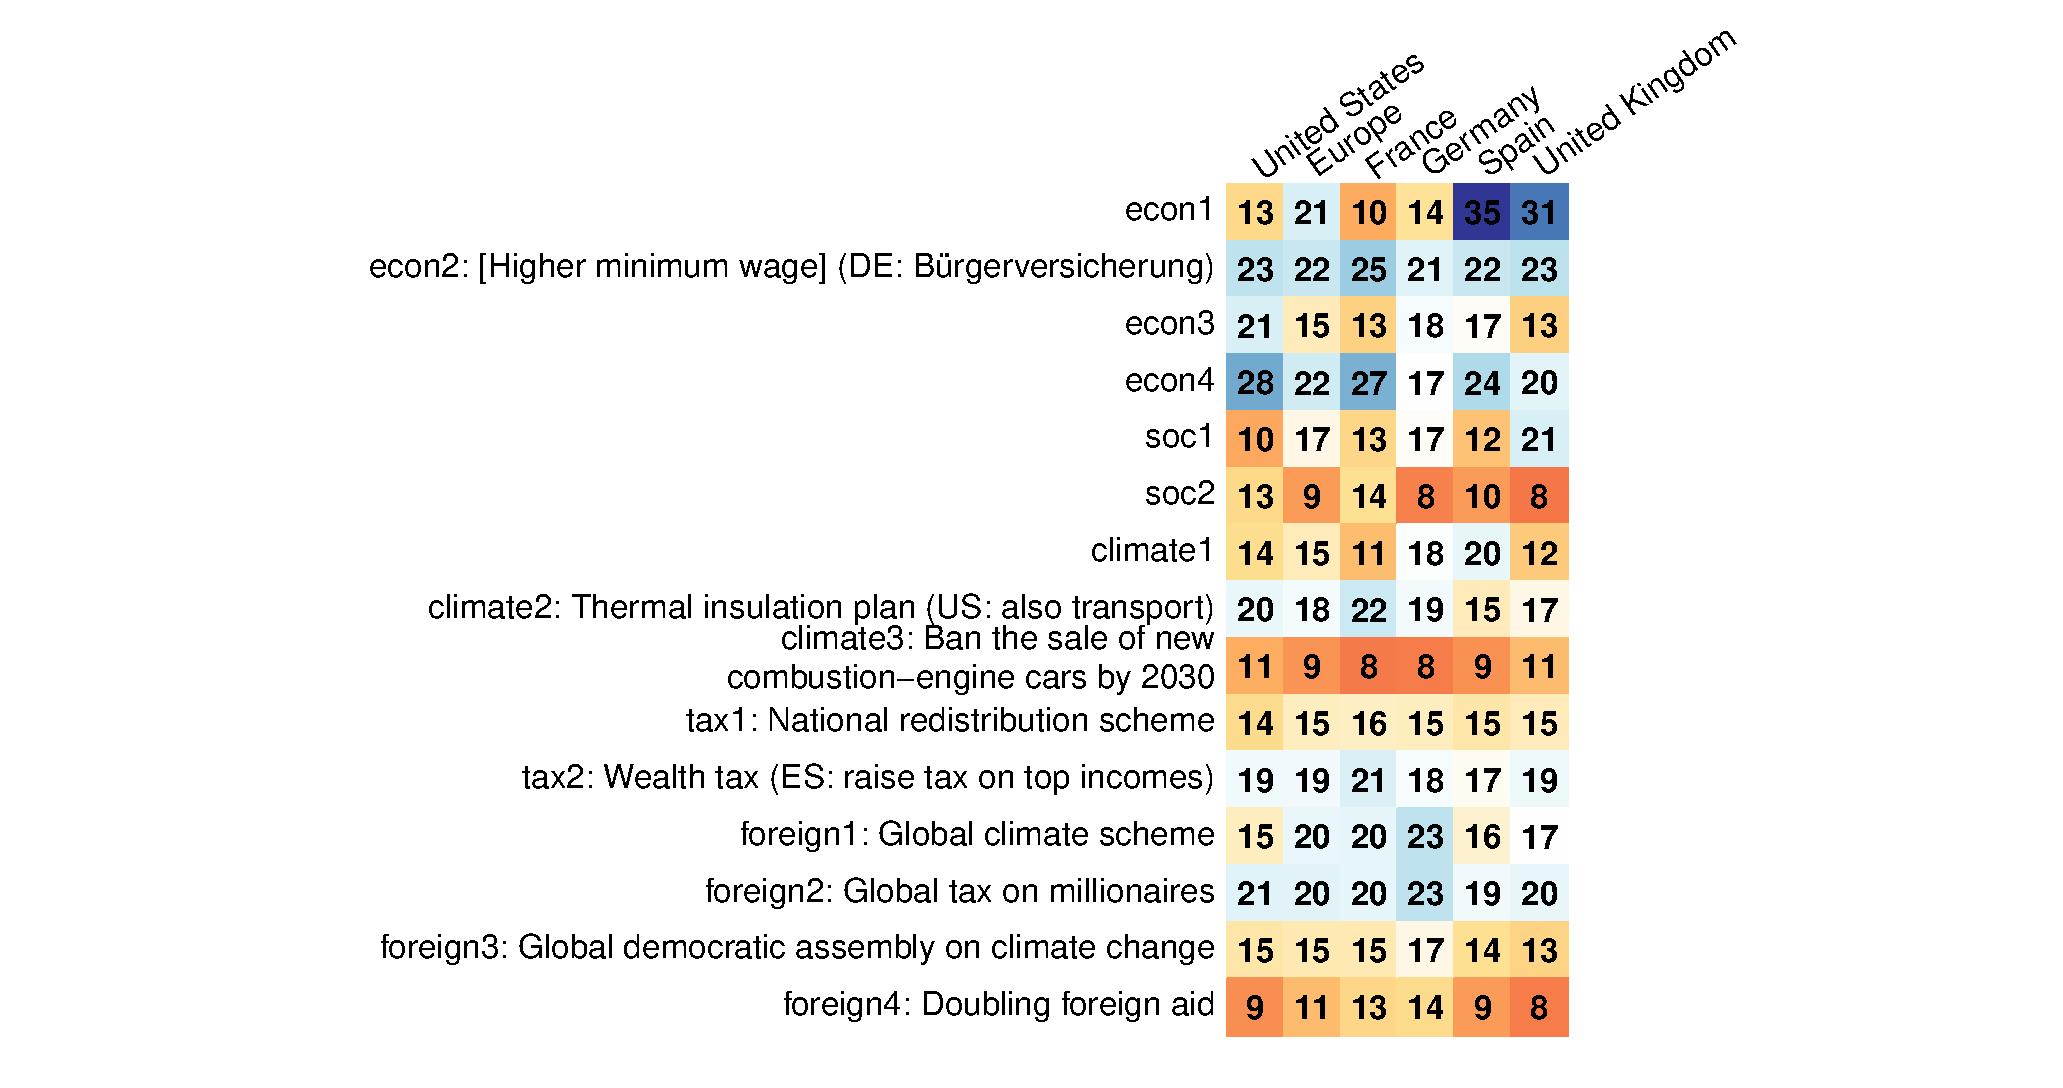
\includegraphics[width=\columnwidth]{../figures/country_comparison/points_mean.pdf} 
%             \end{figure}
%         \end{column}
%     \end{columns}
% \end{frame}

% \begin{frame}{International climate negotiations \hyperlink{donation}{\beamergotobutton{Go back}}\label{negotiation}}
%     \begin{figure}
%         \centering 
%         \caption{In international climate negotiations, would you prefer [U.S.] diplomats to defend [U.S.] interests or global justice?
%         }
%         \vspace{-.2cm}
%         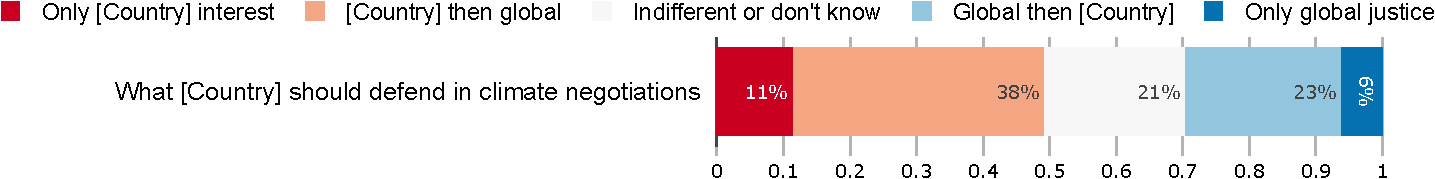
\includegraphics[width=\textwidth]{../figures/all/negotiation.pdf} 
%     \end{figure}
% 	\bbvs \ip The typical answer is to defend one's country's ``interests, to the extent it respects global justice.''
%     \ip Only one eigth wants to defend one's country's ``interests, even if it goes against global justice.''
%     \ee
% \end{frame}

% \begin{frame}{Group defended \hyperlink{donation}{\beamergotobutton{Go back}}\label{group_defended}}
%     \begin{figure}
%         \centering 
%         \caption{What group do you defend when you vote?
%         }
%         \vspace{-.2cm}
%         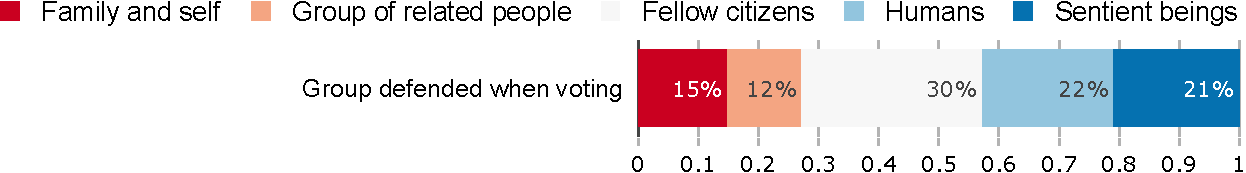
\includegraphics[width=\textwidth]{../figures/all/group_defended_agg2.pdf} 
%     \end{figure}
% 	\bbvs \ip The most defended group is one's fellow citizens.
%     \ip \blue{$~$40\% are universalist}, i.e. defend all humans or sentient beings.
%     \ee
% \end{frame}

% \begin{frame}{Biggest issues \hyperlink{donation}{\beamergotobutton{Go back}}\label{problems}}
%     \begin{figure}
%         \centering 
%         \caption{To what extent do you think the following issues are a problem? \textit{5-Likert scale} \\(Mean of answers recoded in [-2, +2])
%         }
%         \vspace{-.2cm}
%         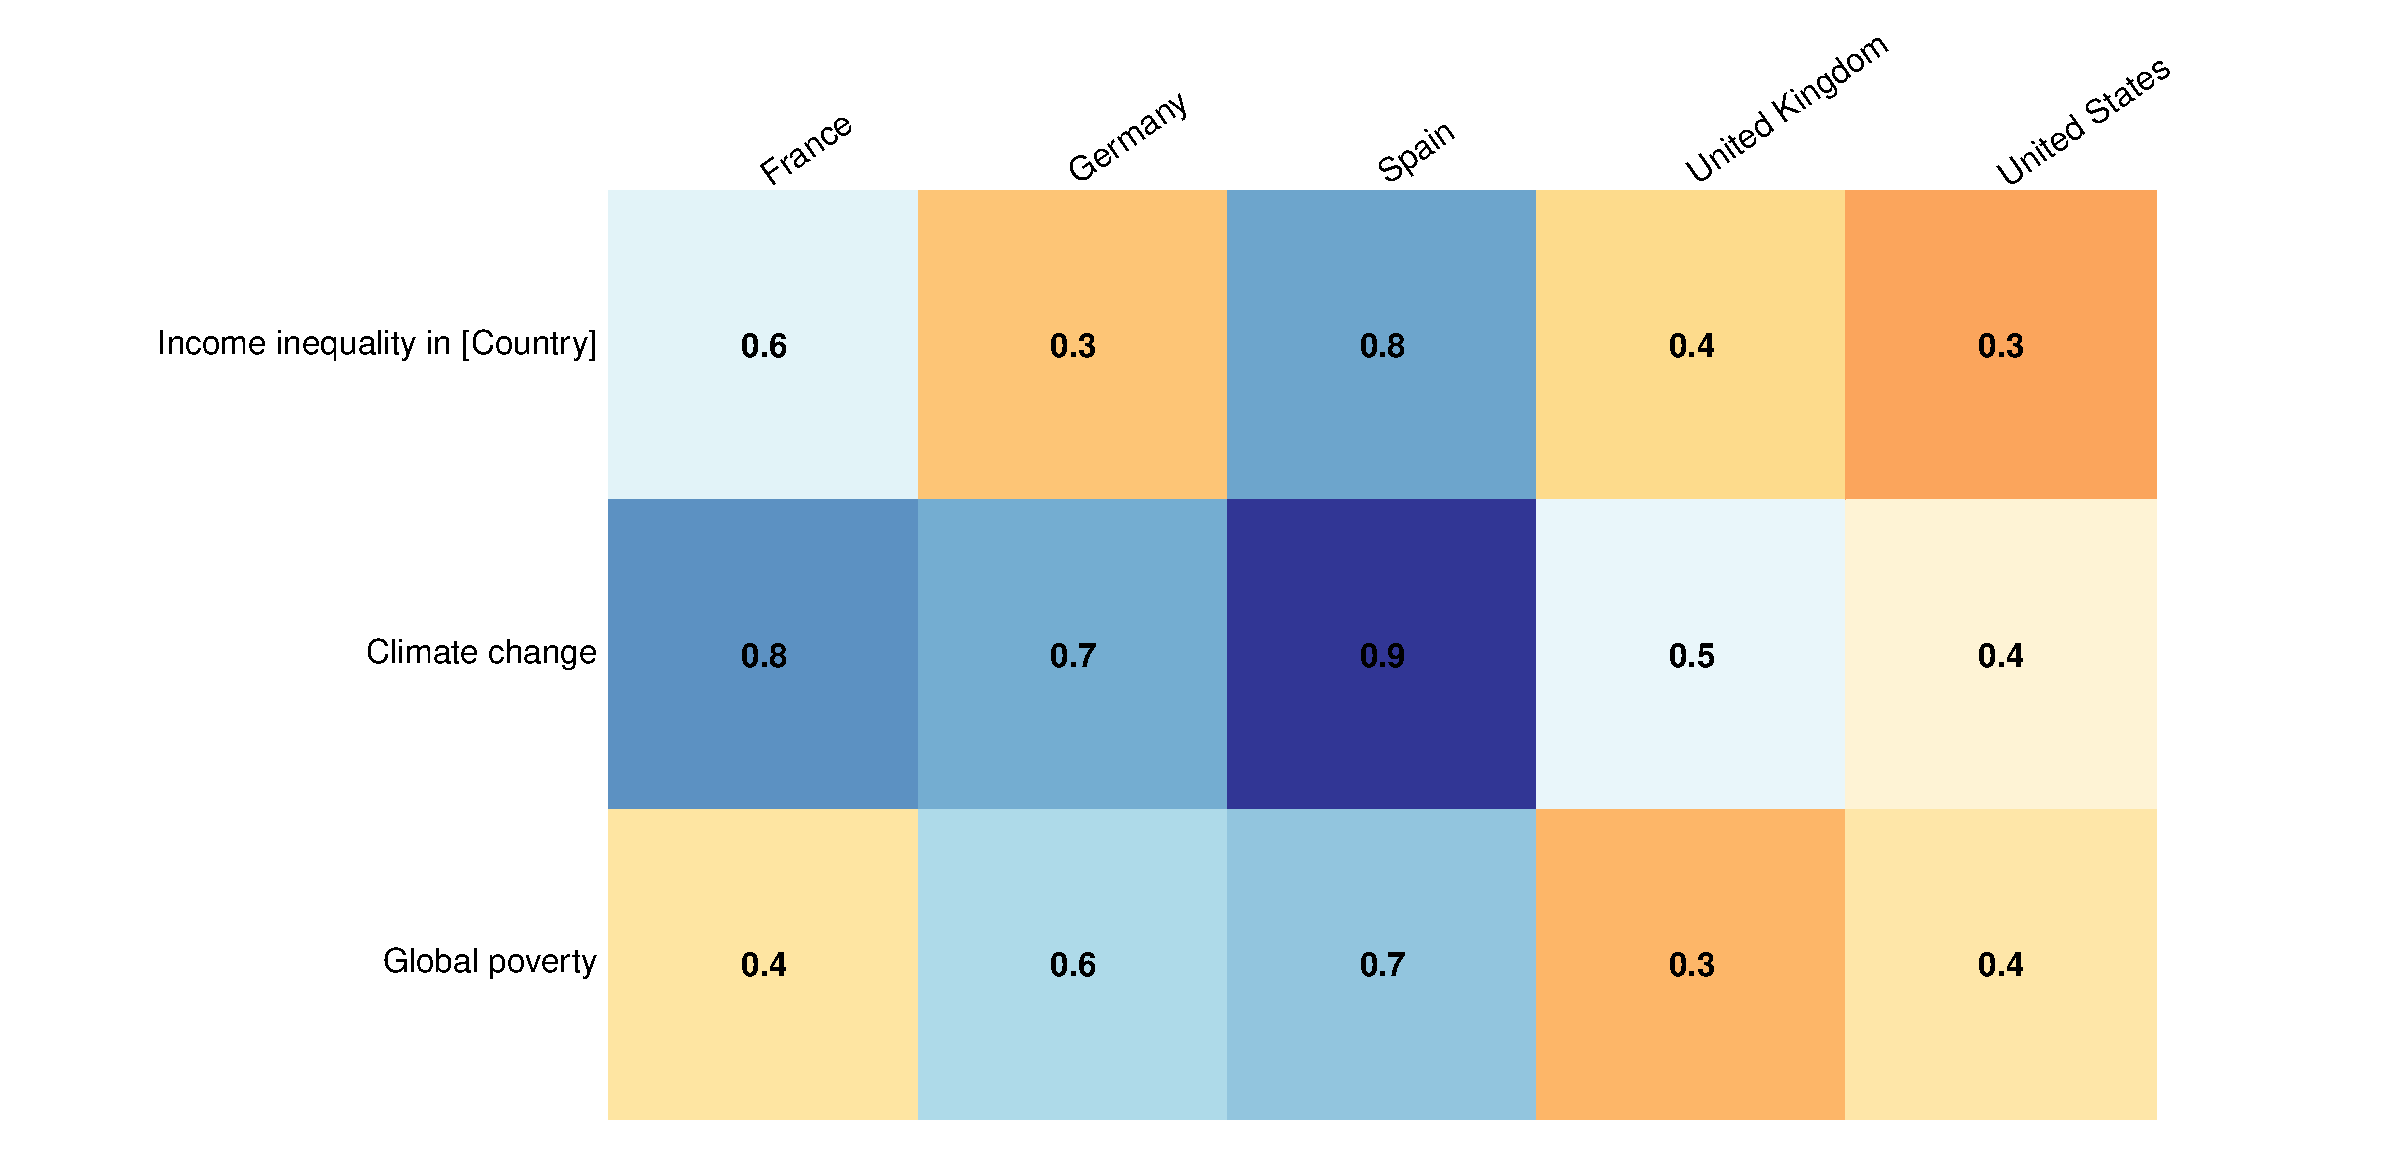
\includegraphics[width=.7\textwidth]{../figures/country_comparison/problem_mean.pdf} 
%     \end{figure}
% 	\bbvs \ip People rank these the importance of these 3 issures as follows: \\ 1. Climate change \\ 2. Global poverty \\ 3. Income inequality in their country
%     \ee
% \end{frame}

% \begin{frame}{Eu questionnaire \hyperlink{questionnaires}{\beamergotobutton{Go back}}\label{survey_flow}}
%     \vspace{.05cm}
%     %\makebox[\textwidth][c]{ 
%     %\begin{itemize}[<+>]
%     \makebox[\textwidth][c]{ 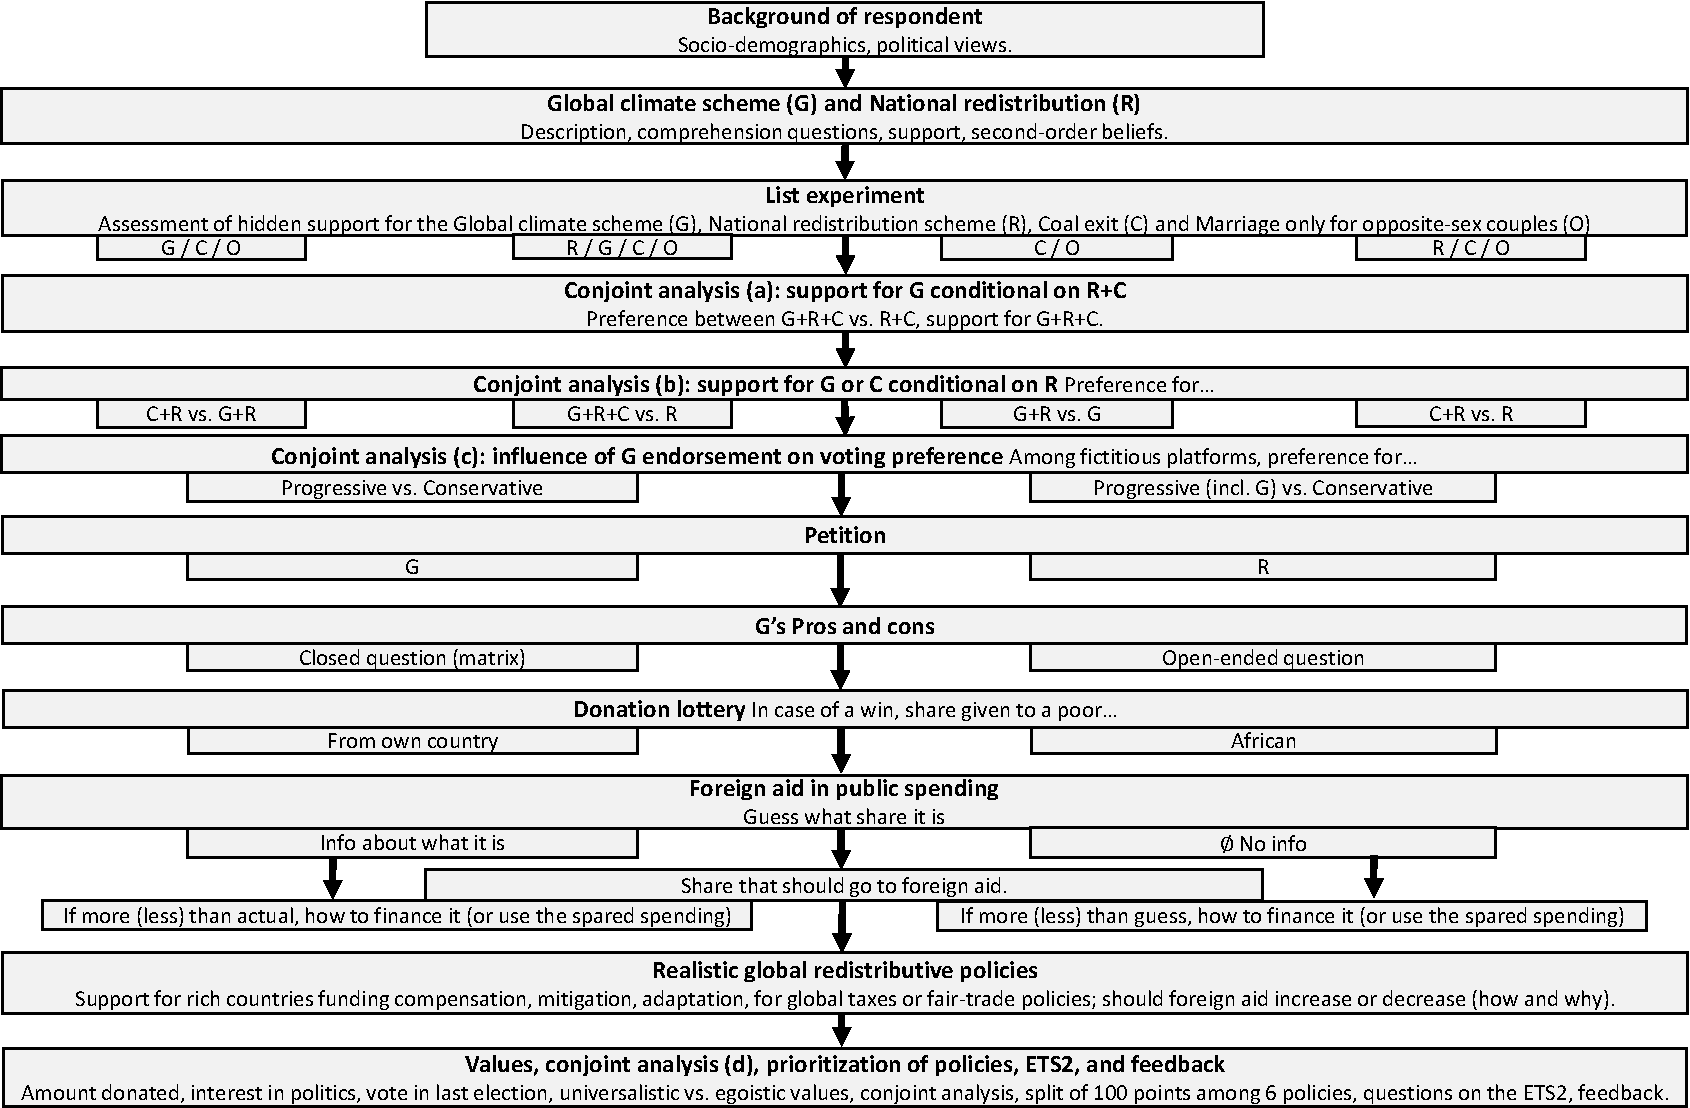
\includegraphics[height=.95\textheight]{../questionnaire/survey_flow_EU.pdf}}
%     %\end{itemize}
%     %}
% \end{frame}

% % \subsection{Representativeness}

% % 	\begin{frame}{Summary statistics\label{representativeness}}	
% % 		\begin{table}[h!]
% % 			\caption{Summary Statistics -- High-income countries 1 }
% % 				\begin{center}
% % 					\scalebox{0.6}{\input{"../tables/sample_composition/AU_CA_DK_FR_ageCombined.tex"}}
% % 				\end{center}
% % 			\end{table}	
% % 	\end{frame}

% % 	\begin{frame}{Summary statistics}	
% % 		\begin{table}[h!]
% % 			\caption{Summary Statistics -- High-income countries 2 \hyperlink{data_quality}{\beamergotobutton{Go back}}}
% % 				\begin{center}
% % 					\scalebox{0.6}{\input{"../tables/sample_composition/DE_IT_JP_PL_ageCombined.tex"}}
% % 				\end{center}
% % 			\end{table}	
% % 	\end{frame}
	
% % \begin{frame}{Summary statistics}	
% % 	\begin{table}[h!]
% % 		\caption{Summary Statistics -- High-income countries 3 \hyperlink{data_quality}{\beamergotobutton{Go back}}}
% % 			\begin{center}
% % 				\scalebox{0.6}{\input{"../tables/sample_composition/SK_SP_UK_US_ageCombined.tex"}}
% % 			\end{center}
% % 		\end{table}	
% % \end{frame}

% \subsection{Descriptive statistics}


% \begin{frame}{Main attitudes by vote \hyperlink{gcs_support}{\beamergotobutton{Go back}}\label{gcs_vote}}
%     \begin{figure}[h!] 
%         \caption{Main attitudes by vote (``Right'' spans from Center-right to Far right). (Relative support in percent)}\label{fig:main_by_vote}
%         \makebox[\textwidth][c]{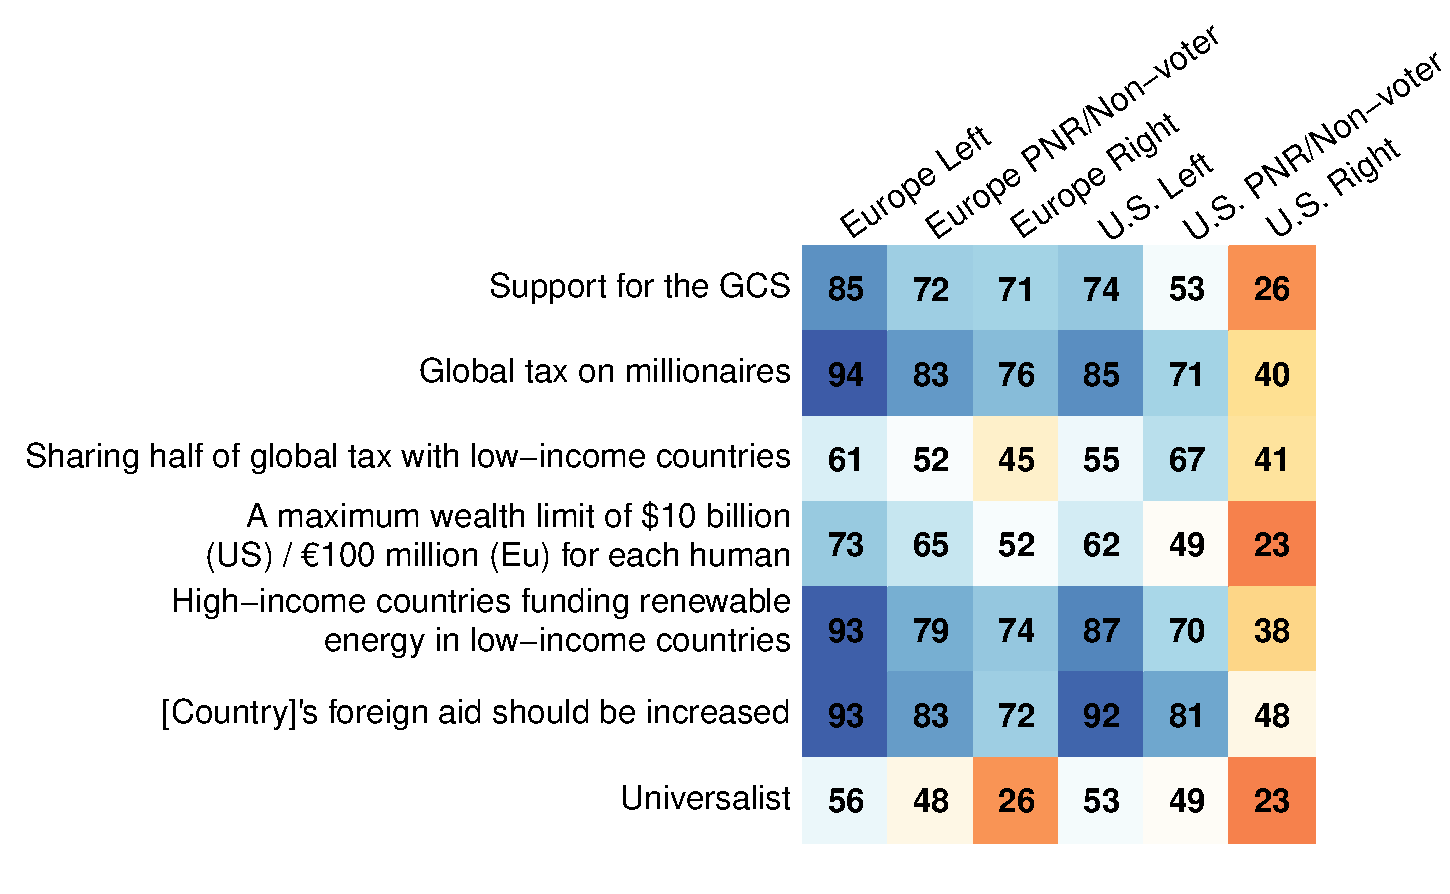
\includegraphics[width=.7\textwidth]{../figures/country_comparison/main_all_by_vote_share.pdf}} 
%     \end{figure}
% \end{frame}

% \begin{frame}{Main attitudes by vote \hyperlink{gcs_support}{\beamergotobutton{Go back}}\label{gcs_vote}} % TODO: Yes on left
%     \begin{figure}[h!] 
%         \only<1>{\caption{Main attitudes by vote in France}
%         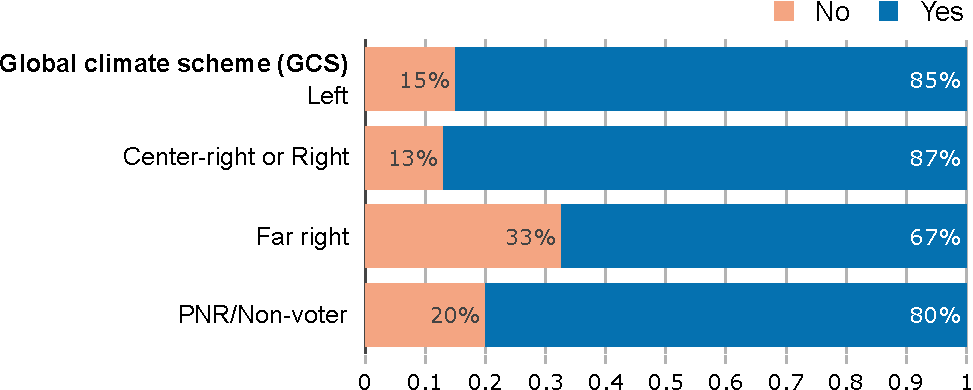
\includegraphics[width=.7\textwidth]{../figures/FR/vote/gcs_support.pdf}}
%         \only<2>{\caption{Main attitudes by vote in Germany}
%         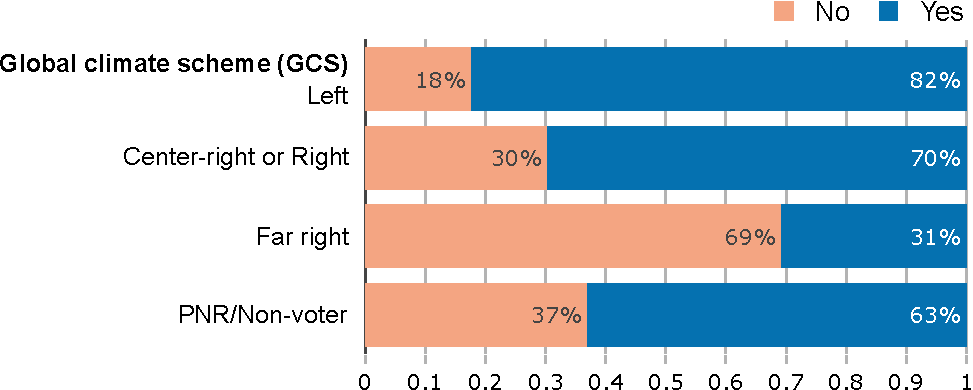
\includegraphics[width=.7\textwidth]{../figures/DE/vote/gcs_support.pdf}}
%         \only<3>{\caption{Main attitudes by vote in Spain}
%         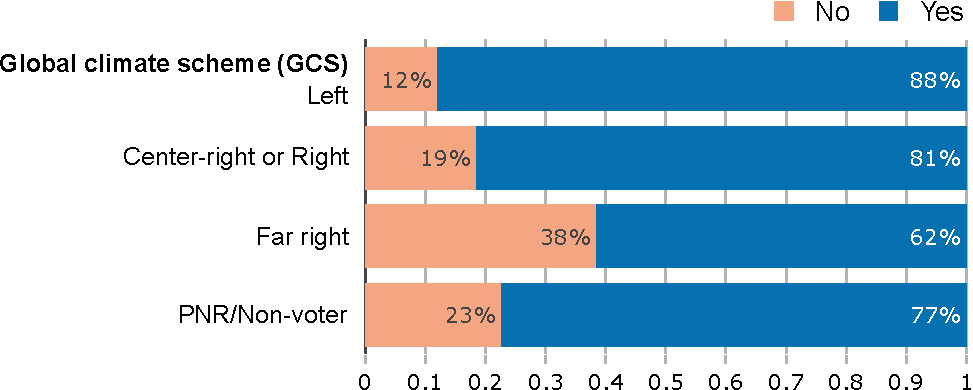
\includegraphics[width=.7\textwidth]{../figures/ES/vote/gcs_support.pdf}}
%         \only<4>{\caption{Main attitudes by vote in the UK}
%         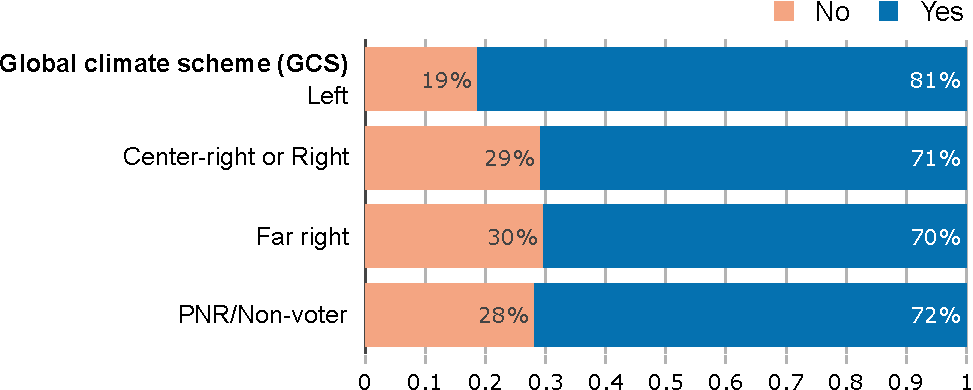
\includegraphics[width=.7\textwidth]{../figures/UK/vote/gcs_support.pdf}}
%     \end{figure}
% \end{frame}

% \begin{frame}{Comprehension of the policies}\label{understanding}
%     \begin{figure}[h!]
%         \caption[Comprehension]{Correct answers to comprehension questions (in percent). \hyperlink{gcs_support}{\beamergotobutton{Go back}}}\label{fig:understood_each}
%         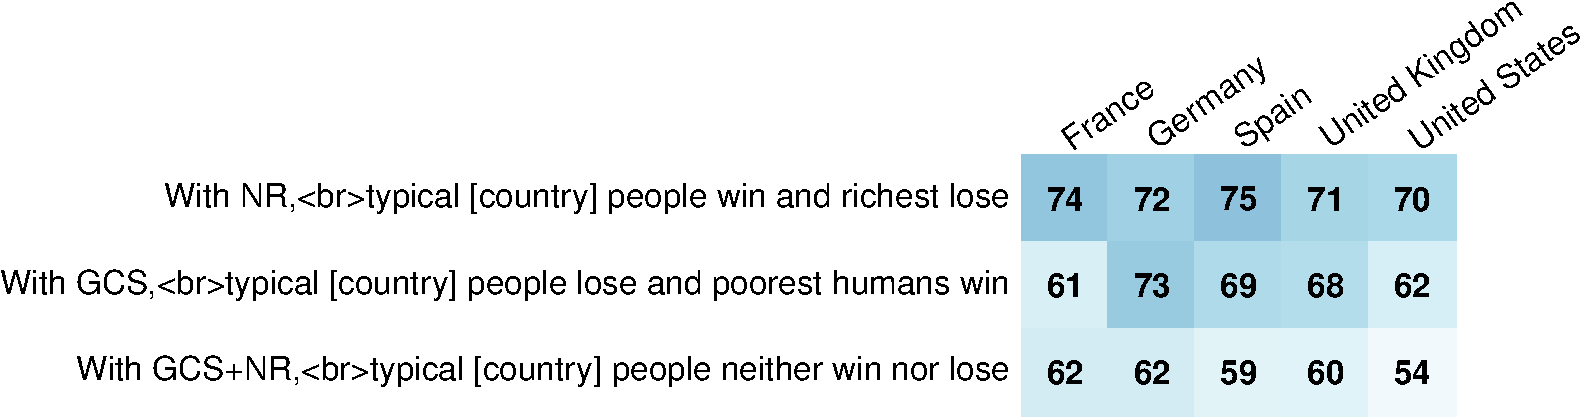
\includegraphics[width=\textwidth]{../figures/country_comparison/understood_each_positive.pdf}
%     \end{figure}    
% \end{frame}

% \begin{frame}{Comprehension of the policies}
% \begin{figure}[h!]
%     \caption[Comprehension score]{Number of correct answers to comprehension questions (mean). \hyperlink{gcs_support}{\beamergotobutton{Go back}}}\label{fig:understood_score}
%     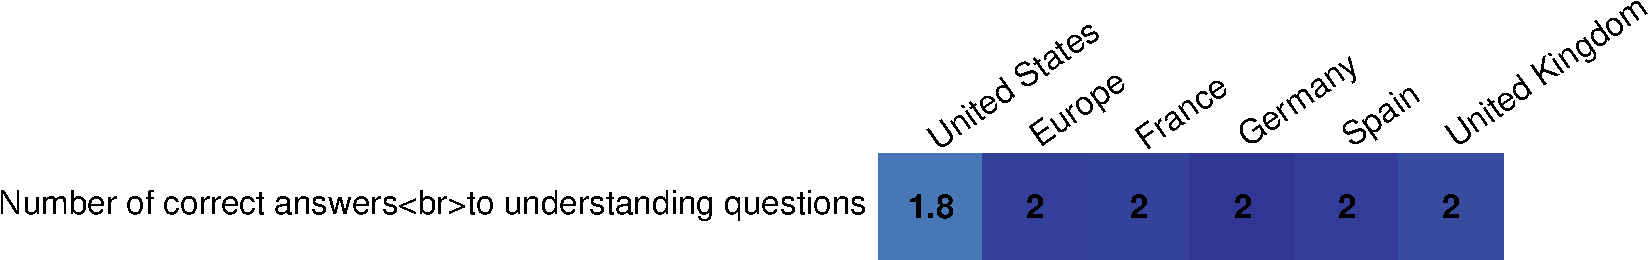
\includegraphics[width=\textwidth]{../figures/country_comparison/understood_score_mean.pdf} 
% \end{figure}
% \end{frame}

% % 
% % 
% % \subsection{Socio-Demographics}
% % \begin{frame}{Education}%\addtocounter{framenumber}{-1} % 
% %     \hspace{.2cm}
% % \begin{figure}[h!]
% % \centering
% % \caption{What is the highest level of education you have completed?}
% % \includegraphics[width=.78\paperwidth]{../../oecd_climate/figures/all/education_ALL} \\
% % \vspace{.3cm}
% % \includegraphics[width=.78\paperwidth]{../../oecd_climate/figures/all/diploma_ALL}
% % %\caption{What race or ethnicity do you identify with? (Multiple answers are possible)} % 
% % %\includegraphics[width=.43\paperwidth]{../../oecd_climate/figures/all/race_ALL}\\
% % \end{figure}
% % \end{frame} % 
% % 
% % \begin{frame}{Left-right leaning}%\addtocounter{framenumber}{-1}
% % \begin{figure}[h!]
% % \centering
% % \caption{On economic policy matters, where do you see yourself on the liberal/conservative spectrum?}
% % \includegraphics[width=.87\paperwidth]{../../oecd_climate/figures/all/left_right_ALL} \\
% % \end{figure}
% % \end{frame}
% % 
% % \begin{frame}{Geography}%\addtocounter{framenumber}{-1}
% % \begin{figure}[h!]
% % \centering
% % \caption{Lives in an urban area (town > 20k people), retrieved from zipcode}
% % \includegraphics[width=.8\paperwidth]{../../oecd_climate/figures/all/urbanity_ALL.png} \\
% % \vspace{.2cm}
% % %\caption{Region, retrieved from zipcode} % 
% % %\includegraphics[width=.43\paperwidth]{../../oecd_climate/figures/all/region_ALL}
% % \end{figure}
% % \end{frame}

% % \begin{frame}{Gender and age}%\addtocounter{framenumber}{-1}
% % \begin{figure}[h!]
% % \centering
% % \caption{What is your gender?}
% % \includegraphics[width=.6\paperwidth]{../../oecd_climate/figures/all/gender_ALL} \\
% % \centering
% % \caption{How old are you?}
% % \includegraphics[width=.6\paperwidth]{../../oecd_climate/figures/all/age_ALL}
% % \end{figure}
% % \end{frame}
% % \subsection{Household %Composition and Energy 
% % Characteristics}

% % \begin{frame}{Income/wealth}%\addtocounter{framenumber}{-1}
% % \begin{figure}[h!]
% % \centering
% % \captionsetup{justification=centering}
% % \caption{What was the annual income of your household in 2019 (before withholding tax, for you and those who live with you)?}
% % \includegraphics[width=.43\paperwidth]{../../oecd_climate/figures/all/income_ALL} \\
% % \caption{\small What is the estimated value of your assets, or the assets of your household if you are married (in [currency])? Include here all your possessions (home, car, savings, etc.) net of debt. For example, if you own a house worth \$300,000 and you have \$100,000 left to repay on your mortgage, your assets are \$200,000.}
% % \includegraphics[width=.43\paperwidth]{../../oecd_climate/figures/all/wealth_ALL} \\
% % \end{figure}
% % \end{frame}


% % \subsection{Political leaning}

% % \begin{frame}{Little interest for politics}%\addtocounter{framenumber}{-1}
% % \vspace{-.5cm}
% % \begin{figure}[h!]
% % \caption{To what extent are you interested in politics?}
% % \includegraphics[width=.52\paperwidth]{../../oecd_climate/figures/all/interested_politics_ALL} \\
% % %\caption{Could you trust the federal goverment to implement the following policies}
% % \vspace{.1cm}
% % \caption{Are you member of an environmental organization?}
% % \includegraphics[width=.47\paperwidth]{../../oecd_climate/figures/all/member_environmental_orga_ALL}\\
% % \vspace{.1cm}
% % \caption{Do you have any relatives who are environmentalists?}
% % \includegraphics[width=.47\paperwidth]{../../oecd_climate/figures/all/relative_environmentalist_ALL}\\
% % \end{figure}
% % \end{frame}

% % \begin{frame}{Broadly representative political leaning}%\addtocounter{framenumber}{-1}
% % \vspace{-.5cm}
% % \begin{figure}[h!]
% % \caption{Did you vote in the [last Country] election?}
% % \includegraphics[width=.45\paperwidth]{../../oecd_climate/figures/all/vote_participation_ALL} \\
% % %\caption{Could you trust the federal goverment to implement the following policies}
% % \vspace{.1cm}
% % \caption{Which candidate did you vote / would you have voted for in the last presidential election?}
% % \includegraphics[width=.7\paperwidth]{../../oecd_climate/figures/all/vote_main_ALL} \\
% % \caption{On economic policy matters, where do you see yourself on the left/right spectrum?}
% % \includegraphics[width=.7\paperwidth]{../../oecd_climate/figures/all/left_right_ALL}
% % % \caption{Which candidate did you vote for in the last presidential election?}
% % % \includegraphics[width=.52\paperwidth]{../../oecd_climate/figures/all/vote_all_ALL} \\
% % % \caption{Did you vote in the 2016 [country] presidential election?}
% % % \includegraphics[width=.47\paperwidth]{../../oecd_climate/figures/all/vote_participation_2016_ALL}\\
% % \end{figure}
% % \end{frame}

% \subsection{Distributive effects of the Global Climate Plan}

% \begin{frame}{Distributive effects of the Global Climate Plan\label{other_distributive} \hyperlink{distributive}{\beamergotobutton{Go back}}}
%     \begin{figure}
%         \centering 
%         \only<1>{ \caption{Distributive effects of the Global Climate Plan in 2030.}
%         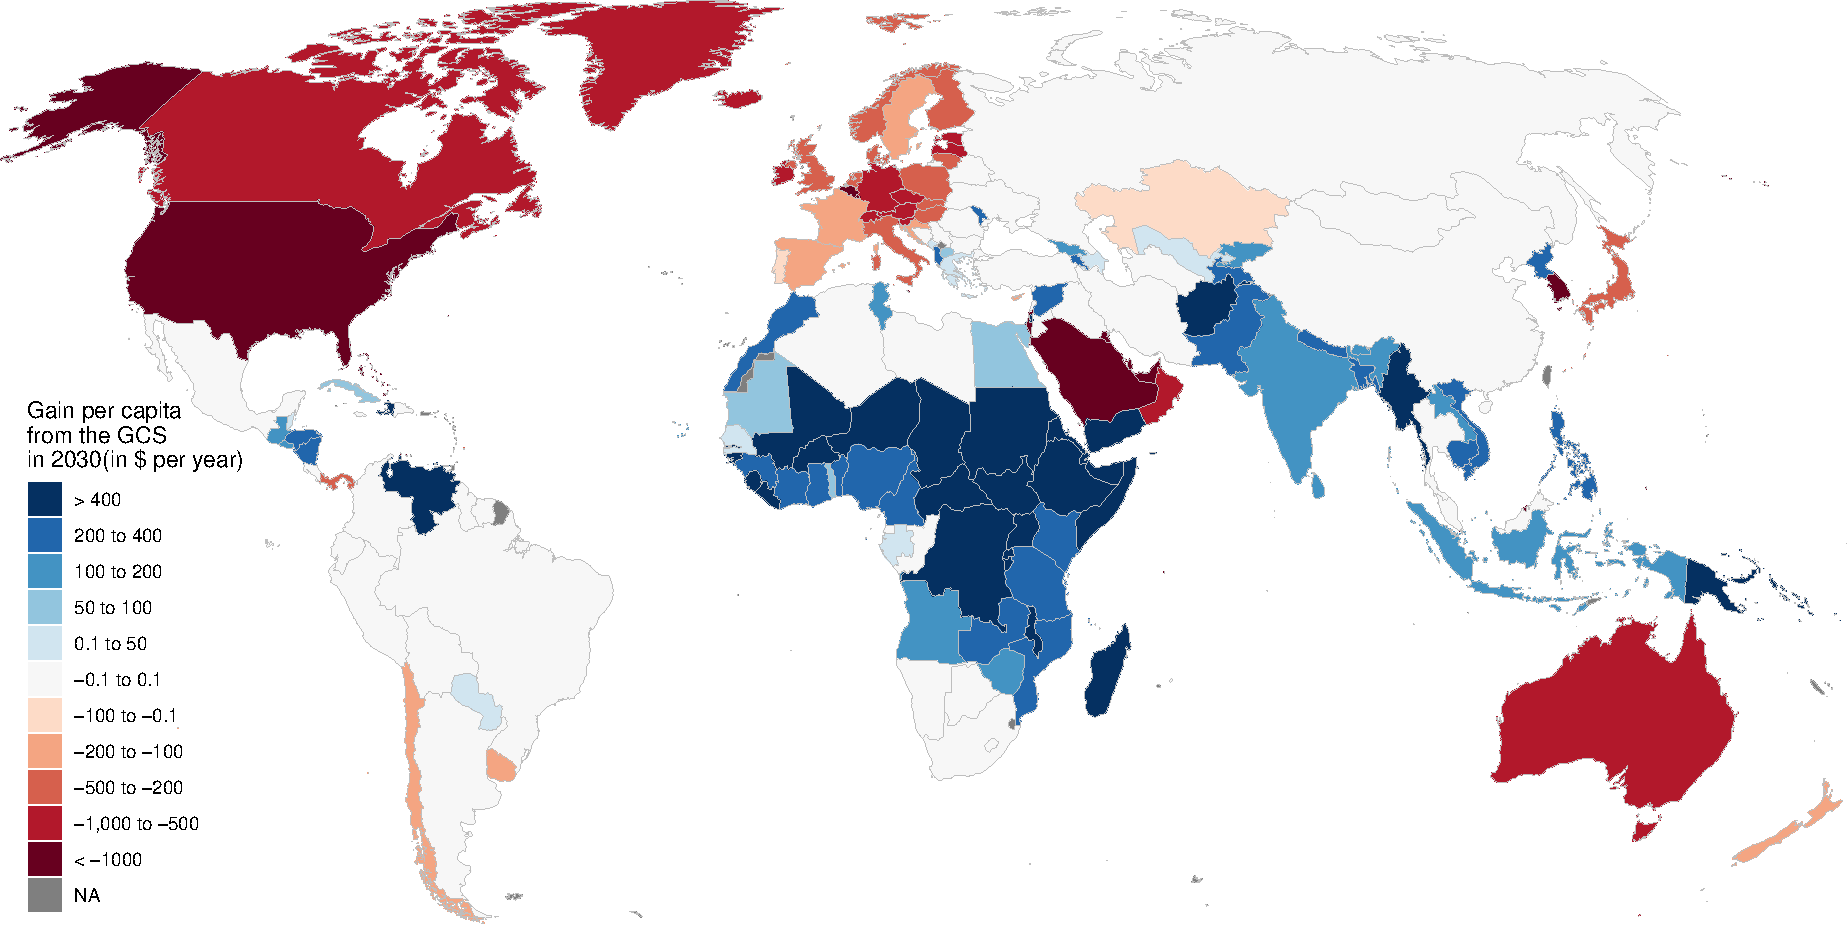
\includegraphics[height=.8\textheight]{../figures/maps/gain_adj_2030.pdf}}
%         \only<2>{ \caption{Distributive effects of the Global Climate Plan in 2040.}
%         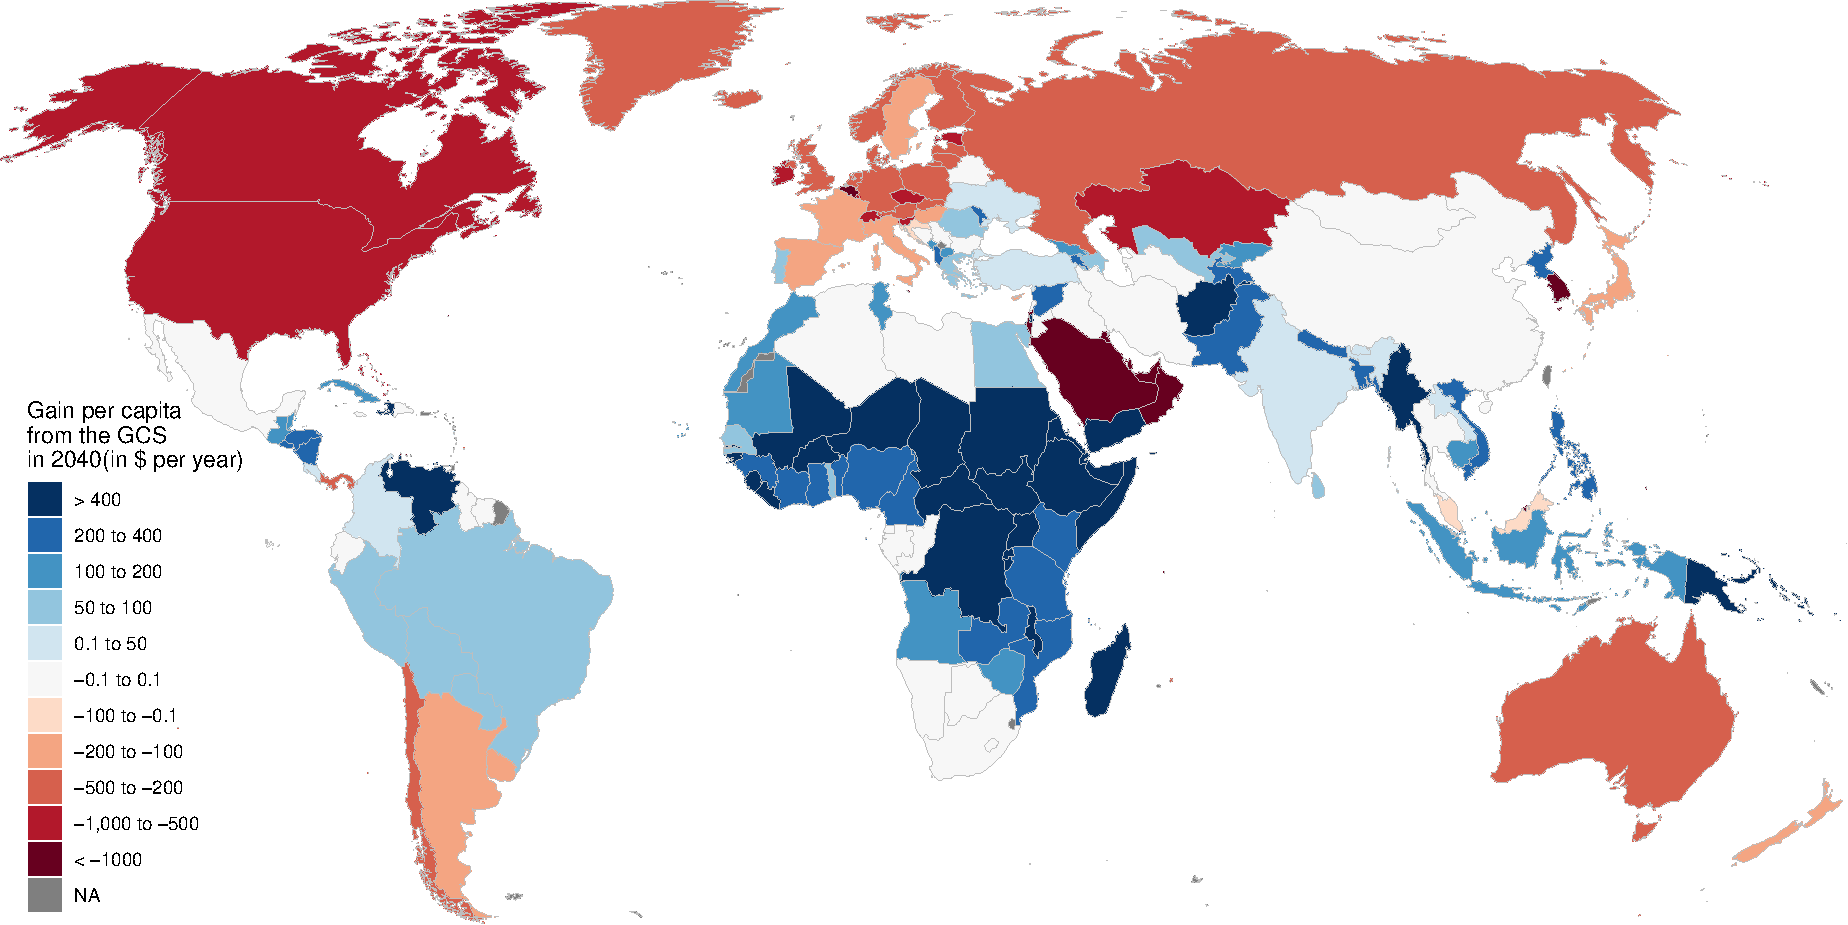
\includegraphics[height=.8\textheight]{../figures/maps/gain_adj_2040.pdf}}
%         \only<3>{ \caption{Distributive effects of the Global Climate Plan in 2050.}
%         \includegraphics[height=.8\textheight]{../figures/maps/gain_adj_2050.pdf}}
%         \only<4>{ \caption{Distributive effects of the Global Climate Plan in 2060.}
%         \includegraphics[height=.8\textheight]{../figures/maps/gain_adj_2060.pdf}}
%         \only<5>{ \caption{Distributive effects of the Global Climate Plan in 2070.}
%         \includegraphics[height=.8\textheight]{../figures/maps/gain_adj_2070.pdf}}
%         \only<6>{ \caption{Distributive effects of the Global Climate Plan in 2080.}
%         \includegraphics[height=.8\textheight]{../figures/maps/gain_adj_2080.pdf}}
%     \end{figure}        
% \end{frame}

% \begin{frame}{Distributive effects of the Global Climate Plan \hyperlink{distributive}{\beamergotobutton{Go back}}}
%     \begin{figure}
%         \centering 
%         \only<1>{ \caption{Distributive effects of the Global Climate Plan in 2030.}
%         \includegraphics[height=.8\textheight]{../figures/maps/gain_adj_over_gdp_2030.pdf}}
%         \only<2>{ \caption{Distributive effects of the Global Climate Plan in 2040.}
%         \includegraphics[height=.8\textheight]{../figures/maps/gain_adj_over_gdp_2040.pdf}}
%         \only<3>{ \caption{Distributive effects of the Global Climate Plan in 2050.}
%         \includegraphics[height=.8\textheight]{../figures/maps/gain_adj_over_gdp_2050.pdf}}
%         \only<4>{ \caption{Distributive effects of the Global Climate Plan in 2060.}
%         \includegraphics[height=.8\textheight]{../figures/maps/gain_adj_over_gdp_2060.pdf}}
%         \only<5>{ \caption{Distributive effects of the Global Climate Plan in 2070.}
%         \includegraphics[height=.8\textheight]{../figures/maps/gain_adj_over_gdp_2070.pdf}}
%         \only<6>{ \caption{Distributive effects of the Global Climate Plan in 2080.}
%         \includegraphics[height=.8\textheight]{../figures/maps/gain_adj_over_gdp_2080.pdf}}
%     \end{figure}        
% \end{frame}

% \begin{frame}{Distributive effects of the Global Climate Plan \hyperlink{distributive}{\beamergotobutton{Go back}}}
%     \begin{figure}
%         \centering 
%         \only<1>{ \caption{Distributive effects of the Global Climate \textit{Scheme}.}
%         \includegraphics[height=.8\textheight]{../figures/maps/npv_over_gdp_gcs.pdf}}
%         \only<2>{ \caption{Distributive effects of the Global Climate \textit{Plan}.}
%         \includegraphics[height=.8\textheight]{../figures/maps/npv_over_gdp_gcs_adj.pdf}}
%         % \only<3>{ \caption{Distributive effects of the Global Climate Plan.}
%         % \includegraphics[height=.8\textheight]{../figures/maps/npv_pa_gcs_adj.pdf}} % TODO! pb with this figure
%     \end{figure}        
% \end{frame}

% \subsection{OECD\label{detail_global}}

% % \begin{frame}{Quasi-unanimous agreement on need for global policies}%\addtocounter{framenumber}{-1}
% % \vspace{-1cm}
% % \begin{figure}[h!]
% % \centering
% % \caption{\small{At which level(s) do you think public policies to tackle climate change need to be put in place? (Multiple answers are possible)}}
% % \includegraphics[width=.43\paperwidth]{../../oecd_climate/figures/all/scale_ALL}
% % \end{figure}
% % \end{frame}

% % \begin{frame}{Large support for international transfers}%\addtocounter{framenumber}{-1}
% % \begin{figure}[h!]
% % \centering
% % \caption{To achieve a given reduction of greenhouse gas emissions globally, costly investments are needed.
% % Ideally, how should countries bear the costs of fighting climate change?}
% % \vspace{2mm}
% % % TODOO \includegraphics[width=.95\paperwidth]{../../oecd_climate/figures/all/burden_sharing_ALL}
% % %\caption{}
% % \end{figure}
% % \end{frame}

% % \begin{frame}{Large support for a fairer global order}%\addtocounter{framenumber}{-1}
% % \begin{figure}[h!]
% % \centering
% % \caption{Do you support or oppose the following policies?}
% % \vspace{2mm}
% % \includegraphics[width=.87\paperwidth]{../../oecd_climate/figures/all/global_policies_ALL}
% % %\caption{}
% % \end{figure}
% % \end{frame}

% \begin{frame}{Relative support for national policies\label{national_policies} \hyperlink{global_policies}{\beamergotobutton{Go back}}} 
%     % National vs. global support: global T&D < national T&D << GCS (except in U.S. where the three are equally supported)
% 	\begin{figure}[h!]
% 	\centering
% 	%\caption{Relative support for national policies}
% 	\includegraphics[height=.8\paperheight]{../../oecd_climate/figures/country_comparison/Heatplot_national_policies_share_countries.pdf}
% 	\end{figure}
%     Support in high-income countries: Global tax and dividend $\lesssim$ National tax and dividend $<$ Global quota and dividend \\ Except in the U.S. where the three are equally supported.
% \end{frame}

% \begin{frame}{Absolute support for global policies\label{absolute_oecd} \hyperlink{global_policies}{\beamergotobutton{Go back}}} 
% \begin{figure}[h!]
%     \centering		
%     \caption{Share of support (somewhat or strongly) for the main global policies among non-\textit{indifferent}.   }
%     \vspace{-.2cm}
%     \includegraphics[height=.82\textheight]{../figures/OECD/Heatplot_global_tax_attitudes_positive.pdf} % burden_share_all_share_countries
%     \end{figure}
% \end{frame}

% \begin{frame}{} % TODOO
% 	\begin{figure}[h!]
% 	\centering
% 	\caption{Do you agree or disagree with the following statement: ``[country] should take measures to fight climate change.'' \hyperlink{global_policies}{\beamergotobutton{Go back}}
% 	%Pourcentage de réponses (plutôt ou très favorable) parmi~:	Très opposé$\cdot$e; Plutôt opposé$\cdot$e; Indifférent$\cdot$e; Plutôt favorable; Très favorable
% 	}
% % \item 
% % 	\\ \textit{Strongly disagree; Somewhat disagree; Neither agree nor disagree; Somewhat agree; Strongly agree}
% 	\includegraphics[height=.8\paperheight]{../../oecd_climate/figures/country_comparison/should_fight_CC_countries.pdf}
% 	\end{figure}
% \end{frame}

% \begin{frame}{}%\addtocounter{framenumber}{-1}
% 	\begin{figure}[h!]
% 	\centering
% 	\caption{
% 		At which level(s) do you think public policies to tackle climate change need to be put in place? (Multiple answers are possible) \hyperlink{global_policies}{\beamergotobutton{Go back}}
% 		%\\ En France, les options sont~: Mondiale; Européenne; Nationale; Locale; 
% 	}
% 		% \begin{enumerate}[resume] \item 
% % \\ \textit{Global; [Federal / European / ...]; [State / National]; Local}
% 	\includegraphics[width=\paperwidth]{../../oecd_climate/figures/country_comparison/scale_positive_countries.pdf}
% 	\end{figure}
% \end{frame}

% \begin{frame}{}
% 	\begin{figure}[h!]
% 	\centering
% 	\caption{How should [country] climate policies depend on what other countries do? \\
% 	If other countries do more, [country] should do... \hyperlink{global_policies}{\beamergotobutton{Go back}}
% 	%Pourcentage de réponse \textit{Plus} ou \textit{Beaucoup plus} parmi~: Beaucoup moins; Moins; À peu près autant; Plus; Beaucoup plus. 
% 	}
% 	% \item How should [country] climate policies depend on what other countries do?
% % 	\begin{itemize}
% % \item If other countries do more, [country] should do…
% % \item If other countries do less, [country] should do…
% % \end{itemize}
% % \textit{Much less; Less; About the same; More; Much more}
% 	\includegraphics[height=.8\paperheight]{../../oecd_climate/figures/country_comparison/if_other_do_more_countries.pdf}
% 	\end{figure}
% \end{frame}

% \begin{frame}{}
% 	\begin{figure}[h!]
% 	\centering
% 	\caption{How should [country] climate policies depend on what other countries do? \\
% 	If other countries do less, [country] should do... \hyperlink{global_policies}{\beamergotobutton{Go back}}
% 	%Pourcentage de réponse \textit{Plus} ou \textit{Beaucoup plus} parmi~: Beaucoup moins; Moins; À peu près autant; Plus; Beaucoup plus.
% 	% Si d'autres pays en font plus, la France devrait en faire...
% 	}
% 	% \item How should [country] climate policies depend on what other countries do?
% % 	\begin{itemize}
% % \item If other countries do more, [country] should do…
% % \item If other countries do less, [country] should do…
% % \end{itemize}
% % \textit{Much less; Less; About the same; More; Much more}
% 	\includegraphics[height=.8\paperheight]{../../oecd_climate/figures/country_comparison/if_other_do_less_countries.pdf}
% 	\end{figure}
% \end{frame}

% % \begin{frame}{}
% % 	\begin{figure}[h!]
% % 	\centering
% % 	\caption{[Question posée seulement aux U.S., au Danemark et en France; ici résultats pour la France] Pour parvenir à une réduction donnée des émissions de gaz à effet de serre au niveau mondial, de coûteux investissements sont nécessaires. \\
% % 	Dans l'idéal, comment les pays devraient-ils répartir les coûts de la lutte contre le changement climatique ? \\
% % 	Pourcentage de réponses (plutôt ou très favorable) parmi~:	Très opposé$\cdot$e; Plutôt opposé$\cdot$e; Indifférent$\cdot$e; Plutôt favorable; Très favorable
% % 	% Les pays devraient payer en proportion de leur richesse
% % 	% Les pays devraient payer en proportion de leurs émissions actuelles
% % 	% Les pays devraient payer en proportion de leurs émissions passées (à partir de 1990)
% % 	% Les pays les plus riches devraient payer davantage, afin que les pays les plus pauvres n'aient pas à payer
% % 	% Les pays les plus riches devraient payer beaucoup plus, pour aider les pays vulnérables à faire face aux conséquences néfastes : les pays vulnérables recevraient de l'argent au lieu de payer
% % 	}
% % % \\ \textit{Strongly oppose; Somewhat oppose; Neither support nor oppose; Somewhat support; Strongly support}
% % % \item ~[In all countries but the U.S., Denmark and France] Suppose the above policy is in place. How should the carbon budget be divided among countries?
% % % \\ \textit{The emission share of a country should be proportional to its population, so that each human has an equal right to emit.; The emission share of a country should be proportional to its current emissions, so that those who already emit more have more rights to emit.; Countries that have emitted more over the past decades (from 1990 onwards) should receive a lower emission share, because they have already used some of their fair share.; Countries that will be hurt more by climate change should receive a higher emission share, to compensate them for the damages.}
% % % \item ~[In the U.S., Denmark, and France only] To achieve a given reduction of greenhouse gas emissions globally, costly investments are needed.
% % % Ideally, how should countries bear the costs of fighting climate change?
% % % 	\begin{itemize}
% % % \item Countries should pay in proportion to their income
% % % \item Countries should pay in proportion to their current emissions
% % % \item Countries should pay in proportion to their past emissions (from 1990 onwards)
% % % \item The richest countries should pay it all, so that the poorest countries do not have to pay anything
% % % \item The richest countries should pay even more, to help vulnerable countries face adverse consequences: vulnerable countries would then receive money instead of paying
% % % \end{itemize} 
% % % \textit{Strongly disagree; Somewhat disagree; Neither agree nor disagree; Somewhat agree; Strongly agree}
% % 	\includegraphics[width=\textwidth]{../../oecd_climate/figures/FR/burden_sharing_FR.png}
% % 	\end{figure}
% % \end{frame}

% \begin{frame}{}
% 	\begin{figure}[h!]
% 	\centering
% 	\caption{\scriptsize [Question non posée aux U.S., au Danemark et en France]  All countries have signed the Paris agreement that aims to contain global warming ``well below +2 \textdegree{}C''. To limit global warming to this level, there is a maximum amount of greenhouse gases we can emit globally, called the carbon budget. Each country could aim to emit less than a share of the carbon budget. To respect the global carbon budget, countries that emit more than their national share would pay a fee to countries that emit less than their share. \\ 
% 	Do you support such a policy? \hyperlink{global_policies}{\beamergotobutton{Go back}}
% 	}
% 	\includegraphics[height=.7\paperheight]{../../oecd_climate/figures/country_comparison/global_quota_countries.pdf}
% 	\end{figure}
% \end{frame}

% \begin{frame}{}
% 	\begin{figure}[h!]
% 	\centering
% 	\caption{[*Question not asked in the U.S., Denmark and France, answers to a similar question are displayed] \\ Suppose the above policy is in place. How should the carbon budget be divided among countries?
% 	\\ The emission share of a country should be proportional to its population, so that each human has an equal right to emit.; The emission share of a country should be proportional to its current emissions, so that those who already emit more have more rights to emit.; Countries that have emitted more over the past decades (from 1990 onwards) should receive a lower emission share, because they have already used some of their fair share.; Countries that will be hurt more by climate change should receive a higher emission share, to compensate them for the damages. \\
% 	Percentage of support (somewhat or strong) among: \textit{Strongly oppose; Somewhat oppose; Neither support nor oppose; Somewhat support; Strongly support} \hyperlink{global_policies}{\beamergotobutton{Go back}}
% 	}
% 	% \item Do you support or oppose establishing a global democratic assembly whose role would be to draft international treaties against climate change? Each adult across the world would have one vote to elect members of the assembly.
% 	\includegraphics[width=\paperwidth]{../../oecd_climate/figures/country_comparison/burden_share_positive_countries.pdf}
% 	\end{figure}
% \end{frame}

% \begin{frame}{}
% 	\begin{figure}[h!]
% 	\centering
% 	\caption{ Do you support or oppose establishing a global democratic assembly whose role would be to draft international treaties against climate change? Each adult across the world would have one vote to elect members of the assembly. \hyperlink{global_policies}{\beamergotobutton{Go back}}
% 	%\\ Pourcentage de réponses (plutôt ou très favorable) parmi~:	Très opposé$\cdot$e; Plutôt opposé$\cdot$e; Indifférent$\cdot$e; Plutôt favorable; Très favorable}
% 	% \item 
% % \\ \textit{Strongly oppose; Somewhat oppose; Neither support nor oppose; Somewhat support; Strongly support
% }
% 	\includegraphics[height=.8\paperheight]{../../oecd_climate/figures/country_comparison/global_assembly_support_countries.pdf}
% 	\end{figure}
% \end{frame}

% \begin{frame}{}
% 	\begin{figure}[h!]
% 	\centering \vspace{-.3cm}
% 	\caption{\scriptsize Imagine the following policy: a global tax on greenhouse gas emissions funding a global basic income. 
% 	Such a policy would progressively raise the price of fossil fuels (for example, the price of gasoline would increase by [40 cents per gallon] in the first years). Higher prices would encourage people and companies to use less fossil fuels, reducing greenhouse gas emissions. Revenues from the tax would be used to finance a basic income of [\$30] per month to each human adult, thereby lifting the 700 million people who earn less than \$2/day out of extreme poverty. 
% 	The average British person would lose a bit from this policy as they would face [\$130] per month in price increases, which is higher than the [\$30] they would receive.
% 	\\
% 	Do you support or oppose such a policy?   \hyperlink{global_policies}{\beamergotobutton{Go back}}
% 	%Pourcentage de réponses (plutôt ou très favorable) parmi~:	Très opposé$\cdot$e; Plutôt opposé$\cdot$e; Indifférent$\cdot$e; Plutôt favorable; Très favorable
% 	}
% % \\ \textit{Strongly oppose; Somewhat oppose; Neither support nor oppose; Somewhat support; Strongly support}
% 	\includegraphics[height=.65\paperheight]{../../oecd_climate/figures/country_comparison/global_tax_support_countries.pdf}
% 	\end{figure}
% \end{frame}

% \begin{frame}{}
% 	\begin{figure}[h!]
% 	\centering
% 	\caption{\scriptsize Do you support or oppose a tax on all millionaires around the world to finance low-income countries that comply with international standards regarding climate action? 
% 	This would finance infrastructure and public services such as access to drinking water, healthcare, and education.  \hyperlink{global_policies}{\beamergotobutton{Go back}}
% 	%Pourcentage de réponses (plutôt ou très favorable) parmi~:	Très opposé$\cdot$e; Plutôt opposé$\cdot$e; Indifférent$\cdot$e; Plutôt favorable; Très favorable
% 	}
% 	% \item D
% % \\ \textit{Strongly oppose; Somewhat oppose; Neither support nor oppose; Somewhat support; Strongly support}
% 	\includegraphics[height=.8\paperheight]{../../oecd_climate/figures/country_comparison/tax_1p_support_countries.pdf}
% 	\end{figure}
% \end{frame}
	
% \begin{frame}{}%\addtocounter{framenumber}{-1}
% 	\begin{figure}[h!]
% 	\centering
% 	\caption{Synthèse~: Pourcentage de réponses positive (e.g. Plutôt/Très favorable). \hyperlink{global_policies}{\beamergotobutton{Go back}}}
% 	\includegraphics[width=\paperwidth]{../../oecd_climate/figures/country_comparison/burden_share_all_positive_countries.pdf}
% 	%\caption{}
% 	\end{figure}
% \end{frame}

% \begin{frame}{}%\addtocounter{framenumber}{-1}
% 	\begin{figure}[h!]
% 	\centering
% 	\caption{Synthèse~: Pourcentage de réponses positive (e.g. \textit{Plutôt/Très favorable}) parmi les non \textit{indifférents}. \hyperlink{global_policies}{\beamergotobutton{Go back}}}
% 	\includegraphics[width=\paperwidth]{../../oecd_climate/figures/country_comparison/burden_share_all_share_countries.pdf}
% 	%\caption{}
% 	\end{figure}
% \end{frame}

	
% \begin{frame}{Principales des attitudes sur les politiques mondiales}%\addtocounter{framenumber}{-1}
% 	\begin{figure}[h!]
% 	\centering
% 	\caption{Pourcentage de réponses positive (e.g. Plutôt/Très favorable). \hyperlink{global_policies}{\beamergotobutton{Go back}}}
% 	\includegraphics[width=\paperwidth]{../../oecd_climate/figures/country_comparison/burden_share_few_positive_countries.pdf}
% 	%\caption{}
% 	\end{figure}
% \end{frame}

% \begin{frame}{Principales attitudes sur les politiques mondiales}%\addtocounter{framenumber}{-1}
% 	\begin{figure}[h!]
% 	\centering
% 	\caption{Pourcentage de réponses positive (e.g. \textit{Plutôt/Très favorable}) parmi les non \textit{indifférents}. \hyperlink{global_policies}{\beamergotobutton{Go back}}}
% 	\includegraphics[width=\paperwidth]{../../oecd_climate/figures/country_comparison/burden_share_few_share_countries.pdf}
% 	%\caption{}
% 	\end{figure}
% \end{frame}

% \begin{frame}{Principales attitudes sur les politiques mondiales}%\addtocounter{framenumber}{-1}
% 	\begin{figure}[h!]
% 	\centering
% 	\caption{Moyennes des réponses, recodées en [$-$2; +2]. \hyperlink{global_policies}{\beamergotobutton{Go back}}}
% 	\includegraphics[width=\paperwidth]{../../oecd_climate/figures/country_comparison/burden_share_few_mean_countries.pdf}
% 	%\caption{}
% 	\end{figure}
% \end{frame}